\documentclass[a4paper,12pt,titlepage]{article}
\usepackage{fancyhdr}
\usepackage{t1enc}
\usepackage[utf8]{inputenc}
\usepackage[magyar]{babel}
\usepackage{lmodern}
\usepackage[pdftex]{graphicx}
\usepackage[lflt]{floatflt}
\usepackage{epstopdf}
\usepackage{amsmath,amssymb}
\usepackage{icomma}
\usepackage{array}
\usepackage[unicode,colorlinks]{hyperref}
\usepackage{fullpage}
\usepackage{booktabs}
\usepackage{subcaption}
\usepackage{mathtools}
\usepackage{physics}
\usepackage{csquotes}
\usepackage[nottoc,numbib]{tocbibind}
\usepackage{float}

\hypersetup{allcolors=black}
\hypersetup{pdfstartview=FitH}
\hypersetup{pdfinfo={
	Title={Szupravezetőbeli spin- és töltéskorrelációk elméleti vizsgálata},
	Author={},
	Subject={},
	Keywords={}
}}


\title{\bf Szupravezetőbeli spin- és töltéskorrelációk elméleti vizsgálata}
\author{Hajdú Csanád \\ \small Témavezető: Dr.\ Zaránd Gergely Attila}
\date{2021.\ 05.\ 21.}
\topmargin = 0pt
\headheight = 14.5pt
\headsep = 14.5pt

\pagestyle{fancy}
\lhead{\small {{Szupravezetőbeli spin- és töltéskorrelációk elméleti vizsgálata} -- 2021.\ 05.\ 21.}}
\rhead{Hajdú Csanád}

\widowpenalty=10000 \clubpenalty=10000

% taken from https://tex.stackexchange.com/a/175245
\makeatletter
\DeclareRobustCommand*\uell{\mathpalette\@uell\relax}
\newcommand*\@uell[2]{
	% We need to adjust the width of \uell to be the same as \ell
	\setbox0=\hbox{$#1\ell$}
	\setbox1=\hbox{\rotatebox{10}{$#1\ell$}}
	\dimen0=\wd0 \advance\dimen0 by -\wd1 \divide\dimen0 by 2
	\mathord{\lower 0.1ex \hbox{\kern\dimen0\unhbox1\kern\dimen0}}
}

\newcommand{\KK}{{\vb*{k}}}
\newcommand{\LL}{{\vb*{\ell}}}
\newcommand{\RR}{{\vb*{r}}}
\newcommand{\phantomdagger}{{\phantom{\dagger}}}
\newcommand{\kF}{{k_\text{F}}}
\newcommand{\EF}{{E_\text{F}}}
\newcommand{\vF}{{v_\text{F}}}
\newcommand{\xic}{{\xi_\text{c}}}

\begin{document}

\begin{titlepage}
\begin{center}
	\vspace*{1cm}
	\textbf{\huge Szupravezetőbeli spin- és töltéskorrelációk elméleti vizsgálata}

	\vspace{1cm}

	BSc szakdolgozat

	\vspace{2.5cm}

	\Large
	Hajdú Csanád

	\vspace{2.5cm}
	{\normalsize Témavezető:} \\
	Dr.\ Zaránd Gergely

	\vfill

	BME Természettudományi Kar \\
	Elméleti Fizika Tanszék

	\vspace{1.5cm}

	2021.\ 05.\ 21.

	\begin{figure}[b]
		\centering
		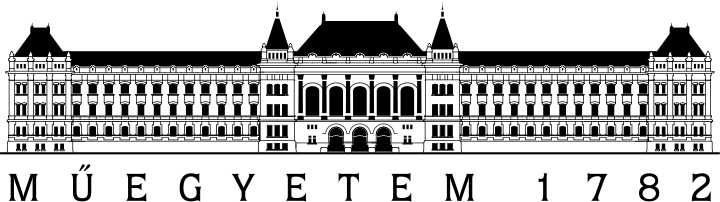
\includegraphics[width=6cm]{bme-logo.png}
	\end{figure}
\end{center}
\end{titlepage}

\null
\thispagestyle{empty}
\addtocounter{page}{-1}
\newpage

\tableofcontents \newpage


% ================================================================
\section{Bevezetés}

A szupravezetést a 20.\ század elején fedezte fel Heike Kamerlingh Onnes holland fizikus, amikor a higany ellenállását vizsgálta alacsony hőmérsékleten.  Azt tapasztalta, hogy $4,2$\,K alatt az ellenállás ugrásszerűen nullára csökkent.  Azóta sok más elemi fémnél és ötvözetnél is tapasztaltak szupravezetést.  Mindegyiknél létezik egy $T_\text{c}$ kritikus hőmérséklet, ami alatt a vezető disszipáció nélkül képes áramot vezetni.  A kritikus hőmérséklet értéke jellemzően $10$\,K alatt van, viszont léteznek olyan anyagok is, amik már $100$\,K körül is szupravezetnek.  Az ilyen anyagokat magas hőmérsékletű szupravezetőknek nevezzük.  Utóbbiak nagy előnye, hogy folyékony hélium helyett folyékony nitrogénnel is lehűthetők annyira, hogy szupravezessenek.

\begin{figure}[h!]
	\centering
	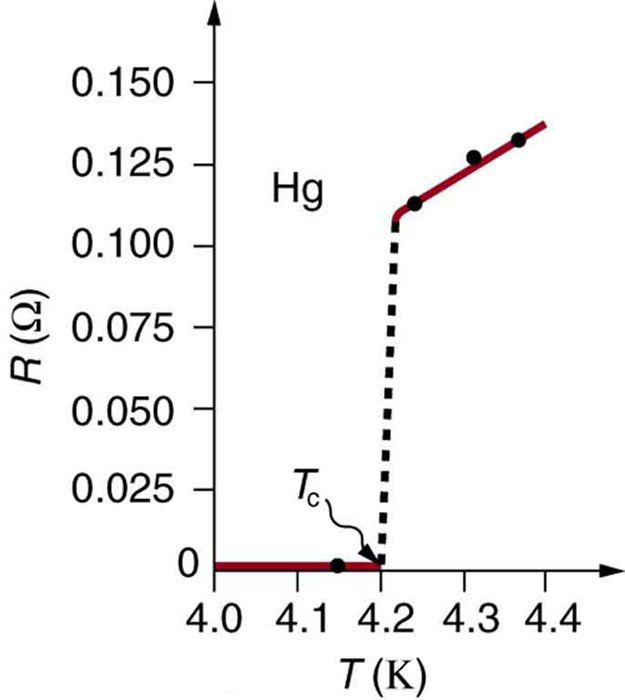
\includegraphics[width=5cm]{higany_R-vs-T.jpg}
	\caption{Egy higany minta ellenállása $T_\text{c}$ körül. \cite{openstax}}
\end{figure}

A szupravezetés jelenségének fontos tulajdonsága a Meissner-effektus, ami egy minta belsejében a mágneses tér teljes kiszorítását jelenti.  Könnyen belátható, hogy egy ideális vezető belsejében a mágneses tér erőssége állandó, a Meissner-effektus viszont ennél nagyobb megszorítást jelent: a minta belsejében a mágneses tér állandó és zérus, még akkor is, ha a szupravezető állapotra egy külső mágneses tér mellett hűtjük le a mintát.

A szupravezetőket széles körben használják.  Az egyik alapvető jelenség, amit felhasználnak a Josephson-effektus, ahol két szupravezető rész közé egy vékony szigetelőt illesztenek és a két vezetőre egy egyenfeszültséget kapcsolnak.  Ekkor a mintán váltóáram mérhető, aminek a frekvenciája $\omega_\text{J} = \frac{2e V}{\hbar}$.  Egy ilyen Josephson-átmenetet használ az úgynevezett SQUID is (superconducting quantum interference device), amivel mágneses tereket lehet nagy pontossággal mérni.  Ezen kívül a Josephson-effektus alapján definiálják az SI rendszerben a volt egységét.  A szupravezetésnek fontos felhasználási területe a nagyterű szupravezető mágnesek, amiket többek között az orvostudományban is használnak MRI készülékekben.  Kvantumszámítógépekben is előnyös szupravezetőket használni a kvantumbitekhez, mivel az energiaspektrumukban lévő gap védelmet biztosít az alacsonyfrekvenciás zaj ellen.

A felfedezése óta számos elmélet született a szupravezetés jelenségének leírására.  A két meghatározó elmélet a Ginzburg--Landau-elmélet, ami egy fenomenologikus elmélet, illetve a BCS-elmélet, ami egy mikroszkopikus leírást ad.
A Ginzburg--Landau-elméletet 1950-ben dolgozták ki Vitaly Ginzburg\footnote{Vitaly Lazarevich Ginzburg, Nobel-díjas (2003) orosz fizikus} és Lev Landau\footnote{Lev Davidovich Landau, Nobel-díjas (1962) orosz fizikus} orosz fizikusok.  Az elmélet jó leírást ad a szupravezetők makroszkopikus tulajdonságaira még olyan anyagoknál is, amikre a BCS-elmélet nem használható.  Ilyenek például a magas hőmérsékletű szupravezetők és a nehéz fermion rendszerek.  Az elméletből ezen kívül levezethető még az első- és másodfajú szupravezetők megkülönböztetése.

A BCS-elméletet John Bardeen\footnote{John Bardeen, kétszeres Nobel-díjas (1956 és 1972) amerikai mérnök és fizikus}, Leon N.\ Cooper\footnote{Leon N.\ Cooper, Nobel-díjas (1972) amerikai fizikus} és John Robert Schrieffer\footnote{John Robert Schrieffer, Nobel-díjas (1972) amerikai fizikus} amerikai fizikusok dolgozták ki, és publikálták 1957-ben.  A BCS-elmélet egy mikroszkopikus leírásmódot ad a szupravezetés jelenségére.  Az elmélet szerint a vezetési elektronok úgynevezett Cooper-párokat alkotnak a köztük lévő, rácsrezgések által közvetített, vonzó kölcsönhatás miatt.  Először Cooper mutatta meg, hogy akármilyen gyenge vonzó kölcsönhatás mellett is a normál állapot instabil lesz, és az elektronok párokba rendeződnek.  Az elektronok párokba rendeződését mérésekkel is igazolni lehet.  A vezető részecskék töltése, így például a Josephson-frekvenciában szereplő töltés is kétszerese az elektron töltésének.

Szupravezetésnél a minta energiaspektrumában megjelenik egy \enquote{rés}, ez az úgynevezett \emph{szupravezető gap}.  Ez a gap a hőmérséklet csökkenésével nő, és $0$\,K-nél éri el a maximumát.  Kialakulása fontos szerepet játszik a szupravezetésben.  Azt tapasztaljuk, hogy ha a gap-et eltüntetjük például egy erős mágneses térrel, akkor a minta már nem szupravezet.  A szupravezető gap értékének hőmérsékletfüggését a \ref{sc-gap}.\ ábrán láthatjuk.  A gap jelenléte azt is jelenti, hogy kevés termikus gerjesztés van a szupravezető állapotban.

\begin{figure}[h!]
	\centering
	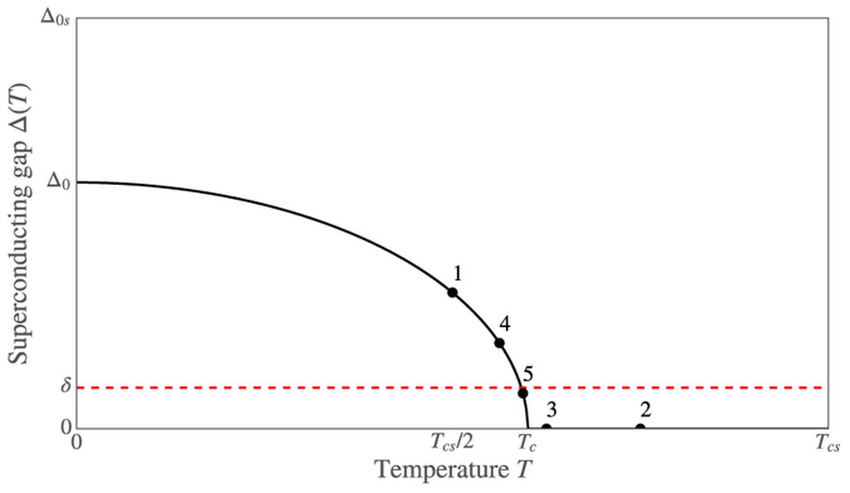
\includegraphics[width=12cm]{sc_gap.png}
	\caption{Szupravezető gap a hőmérséklet függvényében. \cite{superconductor-gap}}
	\label{sc-gap}
\end{figure}

\newpage

A dolgozat célja az, hogy a szupravezető gap jelenléte mellett vizsgáljuk a spin- és töltéskorrelációs függvényeket, és összehasonlítsuk őket a normál állapotban lévő függvényekkel.  Hosszabb távon cél, hogy megértsük egy szupravezetőbe helyezett mágneses szennyezés körül kialakult úgynevezett Kondo-felhőben a spin-korrelációkat.

A dolgozatban először megnézzük a BCS Hamilton-operátor alakját, majd megmutatjuk, hogy ez transzformálható egy olyan alakra, ahol léptetőoperátorok jelennek meg, majd ezekkel a léptetőoperátorokkal felírjuk a korrelációs függvényeket.  Azt fogjuk látni, hogy ezekben két független függvény jelenik meg, amiket kiszámolunk mind normál állapotban, mind szupravezető állapotban.  Ezen függvények aszimptotikus viselkedését is megvizsgáljuk és analitikus közelítő függvényeket adunk meg közel- és távoltérben.  Végül ezek segítségével megkapjuk a spin- és töltéskorrelációs függvényeket normál- és szupravezető állapotban.

A számolásokhoz alapvető kvantumtérelméleti eszközöket használunk, részecske keltő és eltüntető operátorokat, illetve átlagtér közelítést.  Ezen kívül a BCS-elmélet közelítéseivel is élünk.



% ================================================================
\section{Fizikai modell}

\subsection{A BCS Hamilton-operátor}

A BCS-emélet egy egyszerű átlagtér modellt alkalmaz a szupravezetők leírására.  A Hamilton-operátort két részből építi fel, a $H_0$ kinetikus és a $H_\text{int}$ kölcsönhatási tagokból.  A kinetikus tag
\begin{equation}
	H_0 = \sum\limits_\KK \xi_\KK \left( c_{\KK \uparrow}^\dagger c_{\KK \uparrow} + c_{\KK \downarrow}^\dagger c_{\KK \downarrow} \right),
\end{equation}
ahol $c_{\KK \sigma}^\dagger$ a $\left( \KK \sigma \right)$ sajátállapotú elektron keltő operátora és
$$ \xi_\KK = \frac{\hbar^2 k^2}{2 m} - \EF $$
az elektron kinetikus energiája a Fermi-energiához viszonyítva.

A kölcsönhatási tagnál azt a közelítést vesszük, hogy az elektronok csak a Cooper-párokon belül hatnak kölcsön.  Így $H_\text{int}$ felírható úgy, mint a Cooper-párok $\left( \KK \uparrow, -\KK \downarrow \right)$ állapotból $\left( \LL \uparrow, -\LL \downarrow \right)$ állapotba való átmenete,
\begin{equation} \label{H-int-def}
	H_\text{int} = \sum\limits_{\KK, \LL} V_{\KK \LL} \, c_{\LL \uparrow}^\dagger c_{-\LL \downarrow}^\dagger c_{-\KK \downarrow} c_{\KK \uparrow},
\end{equation}
ahol $V_{\KK \LL}$ az átmenet valószínűségi amplitúdója.  A BCS-elméletben ezt a valószínűséget úgy választjuk meg, hogy
$$ V_{\KK \LL} = \left\{ \begin{array}{rl}
	-V, & \text{ha } \left| \xi_\LL \right| < \hbar \omega_\text{D} \text{ és } \left| \xi_\KK \right| < \hbar \omega_\text{D} \\
	0, & \text{egyébként}
\end{array} \right. , $$
ahol $\omega_\text{D}$ a Debeye-frekvencia.  Ez azt jelenti, hogy csak a Fermi-felület közelében lévő elektronok hatnak kölcsön.

Bardeen, Cooper és Schrieffer a Hamilton-operátor alapállapotát a következő variációs hullámfüggvénnyel közelítette,
\begin{equation} \label{phi-tilde}
	\ket{\tilde{\phi}} \equiv \prod\limits_\KK \left( u_\KK + v_\KK \, c_{\KK \uparrow}^\dagger c_{-\KK \downarrow}^\dagger \right) \ket{0},
\end{equation}
ahol a $\ket{0}$ vákuum állapotba helyezünk be Cooper-párokat valamilyen amplitúdóval.  Az $u_\KK$ és $v_\KK$ együtthatók általános esetben komplexek és ahhoz, hogy $\ket{\tilde{\phi}}$ normálva legyen teljesülnie kell az
\begin{equation} \label{u-v-norm}
	\left| u_\KK \right|^2 + \left| v_\KK \right|^2 = 1
\end{equation}
relációnak.  Ezzel a formalizmussal a normál állapot hullámfüggvényét is felírhatjuk, ahol minden elektronállapot be van töltve a Fermi-felületig,
\begin{equation}
	\ket{\tilde{\phi}_\text{n}} = \prod\limits_{\left| \KK \right| < \kF} c_{\KK \uparrow}^\dagger c_{-\KK \downarrow}^\dagger \ket{0},
\end{equation}
ez az
\begin{equation} \label{u-v-normal}
	u_\KK = \left\{ \begin{array}{ll} 0, & \text{ha } \left| \KK \right| < \kF \\ 1, & \text{ha } \left| \KK \right| > \kF \end{array} \right.
	~~~ \text{és} ~~~
	v_\KK = \left\{ \begin{array}{ll} 1, & \text{ha } \left| \KK \right| < \kF \\ 0, & \text{ha } \left| \KK \right| > \kF \end{array} \right.
\end{equation}
együtthatóknak felel meg.

A \eqref{H-int-def}-ben lévő kölcsönhatást átlagtér közelítéssel átírhatjuk,
\begin{equation}
	c_{\LL \uparrow}^\dagger c_{-\LL \downarrow}^\dagger c_{-\KK \downarrow} c_{\KK \uparrow} \approx \expval{c_{\LL \uparrow}^\dagger c_{-\LL \downarrow}^\dagger} c_{-\KK \downarrow} c_{\KK \uparrow} + c_{\LL \uparrow}^\dagger c_{-\LL \downarrow}^\dagger \expval{c_{-\KK \downarrow}^\phantomdagger c_{\KK \uparrow}^\phantomdagger} - \expval{c_{\LL \uparrow}^\dagger c_{-\LL \downarrow}^\dagger} \expval{c_{-\KK \downarrow}^\phantomdagger c_{\KK \uparrow}^\phantomdagger}.
\end{equation}
Ezen kívül vezessük be a $\Delta_\KK$ mennyiséget,
\begin{equation}
	\Delta_\KK^* \equiv \left\{ \begin{array}{ll}
	V \, {\sum\limits_\LL}^\prime \expval{c_{\LL \uparrow}^\dagger c_{-\LL \downarrow}^\dagger}, & \text{ha } \left| \xi_\KK \right| < \hbar \omega_\text{D} \\
	0, & \text{egyébként}
	\end{array} \right. ,
\end{equation}
ahol ${\sum_\LL}^\prime$ azt jelöli, hogy az összegzés csak a $\left| \xi_\LL \right| < \hbar \omega_\text{D}$ állapotokra történik.  Ezután a fenti átlagtér közelítést alkalmazva \eqref{H-int-def} a következőképp közelíthető,
\begin{equation}
	H_\text{int} \approx - \sum\limits_\KK \left( \Delta_\KK c_{\KK \uparrow}^\dagger c_{-\KK \downarrow}^\dagger + \Delta_\KK^* c_{-\KK \downarrow} c_{\KK \uparrow} \right) + \text{cst}.
\end{equation}

Ezzel felírhatjuk a teljes BCS Hamilton-operátort,
\begin{equation}
	H_\text{BCS} = H_0 + H_\text{int} \approx \sum\limits_\KK \left[ \xi_\KK \left( c_{\KK \uparrow}^\dagger c_{\KK \uparrow} + c_{\KK \downarrow}^\dagger c_{\KK \downarrow} \right) - \Delta_\KK c_{\KK \uparrow}^\dagger c_{-\KK \downarrow}^\dagger - \Delta_\KK^* c_{-\KK \downarrow} c_{\KK \uparrow} \right] + \text{cst}.
\end{equation}


\subsection{Az szupravezető-állapot léptetőoperátorai}

A BCS Hamilton-operátor spektrumának meghatározásához azt léptetőoperátorok segítségével fejezzük ki,
\begin{equation} \label{H-BCS}
	H_\text{BCS} = \sum\limits_\KK E_\KK \left( \gamma_{\KK \uparrow}^\dagger \gamma_{\KK \uparrow} + \gamma_{\KK \downarrow}^\dagger \gamma_{\KK \downarrow} \right) + \text{cst},
\end{equation}
ahol a $\gamma_{\KK \sigma}$ operátorok a szupravezető-állapot kvázirészecskéinek léptetőoperátorai.  Ezek kielégítik a következő relációkat,
\begin{equation} \label{gamma-anticommutator}
\begin{split}
	\anticommutator{\gamma_{\KK \sigma}^\phantomdagger}{\gamma_{\KK^\prime \sigma^\prime}^\phantomdagger} & = \anticommutator{\gamma_{\KK \sigma}^\dagger}{\gamma_{\KK^\prime \sigma^\prime}^\dagger} = 0, \\
	\anticommutator{\gamma_{\KK \sigma}^\phantomdagger}{\gamma_{\KK^\prime \sigma^\prime}^\dagger} & = \delta_{\KK \KK^\prime} \delta_{\sigma \sigma^\prime},
\end{split}
\end{equation}
ahol $\anticommutator{A}{B} = AB + BA$ az antikommutátor.  Az alapállapotot az eltüntető operátoroknak a nullelembe kell vinniük, vagyis
\begin{equation} \label{gamma-zero}
	\gamma_{\KK \sigma} \ket{\tilde{\phi}} = 0.
\end{equation}

Megmutatható, hogy a
\begin{equation} \label{gamma-def}
\begin{split}
	\gamma_{\KK \uparrow} & = u_\KK c_{\KK \uparrow} - v_\KK c_{-\KK \downarrow}^\dagger \\
	\gamma_{\KK \downarrow} & = u_\KK c_{\KK \downarrow} + v_\KK c_{-\KK \uparrow}^\dagger
\end{split}
\end{equation}
választással teljesülnek a \eqref{gamma-anticommutator} és \eqref{gamma-zero} összefüggések.

A $\gamma_{\KK \sigma}$ operátorokra kapott \eqref{gamma-def} kifejezést invertálva megkaphatjuk a $c_{\KK \sigma}$ operátorokat is,
\begin{equation}
\begin{split}
	c_{\KK \uparrow} & = u_\KK^* \gamma_{\KK \uparrow} + v_\KK \gamma_{-\KK \downarrow}^\dagger, \\
	c_{\KK \downarrow} & = u_\KK^* \gamma_{\KK \downarrow} - v_\KK \gamma_{-\KK \uparrow}^\dagger.
\end{split}
\end{equation}


\subsection{Az $u_\KK$ és $v_\KK$ együtthatók meghatározása}

Az $u_\KK$ és $v_\KK$ együtthatók meghatározásához a léptetőoperátorok tulajdonságait használjuk fel.  A \eqref{H-BCS} egyenletből következik, hogy
\begin{equation} \label{H-gamma-commutator}
	\commutator{H_\text{BCS}}{\gamma_{\KK \uparrow}^\dagger} = E_\KK \gamma_{\KK \uparrow}^\dagger.
\end{equation}
A $\commutator{H_\text{BCS}}{\gamma_{\KK \uparrow}^\dagger}$ kommutátor kiszámolásához használjuk fel a \eqref{gamma-def} összefüggést, tehát számoljuk ki egyenként $\commutator{H_\text{BCS}}{c_{\KK \uparrow}^\dagger}$ és $\commutator{H_\text{BCS}}{c_{-\KK \downarrow}}$ értékét.  A $c_{\KK \sigma}$ operátorok felcserélési relációjából könnyen belátható, hogy
\begin{equation}
	\commutator{H_\text{BCS}}{c_{\KK \uparrow}^\dagger} = \xi_\KK c_{\KK \uparrow}^\dagger - \Delta_\KK^* c_{-\KK \downarrow}
\end{equation}
és
\begin{equation}
	\commutator{H_\text{BCS}}{c_{-\KK \downarrow}} = -\xi_\KK c_{-\KK \downarrow} - \Delta_\KK c_{\KK \uparrow}^\dagger.
\end{equation}
Így a \eqref{H-gamma-commutator} összefüggés tovább írható,
\begin{equation}
	u_\KK^* \left( \xi_\KK c_{\KK \uparrow}^\dagger - \Delta_\KK^* c_{-\KK \downarrow} \right) - v_\KK^* \left( -\xi_\KK c_{-\KK \downarrow} - \Delta_\KK c_{\KK \uparrow}^\dagger \right) = E_\KK \left( u_\KK^* c_{\KK \uparrow}^\dagger - v_\KK^* c_{-\KK \downarrow} \right),
\end{equation}
amit egy lineáris egyenletrendszerként is felírhatunk,
\begin{equation}
	\begin{pmatrix}
		\xi_\KK & \Delta_\KK \\
		\Delta_\KK^* & -\xi_\KK
	\end{pmatrix} \begin{pmatrix} u_\KK^* \\ v_\KK^* \end{pmatrix}
	= E_\KK \begin{pmatrix} u_\KK^* \\ v_\KK^* \end{pmatrix}.
\end{equation}
A sajátértékekre $E_\KK = \pm \sqrt{\xi_\KK^2 + \left| \Delta_\KK \right|^2}$ adódik, amiből a pozitív előjelű feleltethető meg a felfelé léptető operátornak.  Végül az $u_\KK$ és $v_\KK$ együtthatókra, figyelembe véve a \eqref{u-v-norm} normálási feltételt,
\begin{equation} \label{u-v-sc}
	u_\KK = \frac{\Delta_\KK^*}{\sqrt{2 E_\KK \left( E_\KK - \xi_\KK \right)}} ~~~ \text{és} ~~~ v_\KK = \frac{E_\KK - \xi_\KK}{\sqrt{2 E_\KK \left( E_\KK - \xi_\KK \right)}}
\end{equation}
adódik.


\subsection{Levágási séma}

A BCS-elméletben $\Delta_\KK$ definíciója
\begin{equation}
	\Delta_\KK = \Delta(\xi_\KK) = \left\{ \begin{array}{cl} \Delta, & \text{ha } \left| \xi_\KK \right| < \hbar \omega_\text{D} \\ 0, & \text{ha } \left| \xi_\KK \right| > \hbar \omega_\text{D} \end{array} \right. ,
\end{equation}
ahol $\omega_\text{D}$ a Debeye-frekvencia.  Ez azt jelenti, hogy csak a Fermi-felület közelében lévő elektronok vesznek részt a szupravezetésben.

E helyett az éles levágás helyett mi egy sima függvényt használunk, így a számolás során kapott integrálokat egyszerűbben tudjuk kezelni.  A használt levágás
\begin{equation} \label{cutoff}
	w(\xi) = \frac{1}{\left( \frac{\xi}{\hbar \omega_\text{D}} \right)^4 + 1}
\end{equation}
alakú, ami az éles levágáshoz hasonlóan nagyjából a $\left[ -\hbar \omega_\text{D}, \hbar \omega_\text{D} \right]$ tartományon nem zérus. A szupravezető gap impulzus- és energiafüggését mi is elhanyagoljuk, értékét konstans $\Delta$-nak választjuk.  A legtöbb szupravezetőben $\left|\Delta\right| \ll \hbar \omega_\text{D} \ll \EF$, amit a számolásaink során ki is fogunk használni.



% ================================================================
\section{Korrelátorok számítása}

A korrelátorok kiszámításához a $\psi_\sigma(\RR)$ téroperátorokat használjuk.  Ezek a $c_{\KK \sigma}$ operátorokhoz hasonlóan eltüntető operátorok, viszont $\psi_\sigma(\RR)$ egy $\left( \KK \sigma \right)$ sajátállapotú részecske helyett egy $\left( \RR \sigma \right)$ sajátállapotút tüntet el az állapotfüggvényből.  A téroperátorokat kifejezhetjük a korábban meghatározott kvázirészecske operátorokkal,
\begin{equation} \label{psi}
\begin{split}
	\psi_\uparrow(\RR) & = \frac{1}{\sqrt{V}} \sum\limits_\KK e^{i \KK \RR} c_{\KK \uparrow} = \frac{1}{\sqrt{V}} \sum\limits_\KK e^{i \KK \RR} \left( u_\KK^* \gamma_{\KK \uparrow} + v_\KK \gamma_{-\KK \downarrow}^\dagger \right), \\
	\psi_\downarrow(\RR) & = \frac{1}{\sqrt{V}} \sum\limits_\KK e^{i \KK \RR} c_{\KK \downarrow} = \frac{1}{\sqrt{V}} \sum\limits_\KK e^{i \KK \RR} \left( u_\KK^* \gamma_{\KK \downarrow} - v_\KK \gamma_{-\KK \uparrow}^\dagger \right).
\end{split}
\end{equation}

A téroperátorok segítségével kifejezhetjük a töltés- és spinsűrűség operátorokat,
\begin{equation} \label{charge-density}
	e \, \rho(\RR) = e \left( \psi_\uparrow^\dagger(\RR) \psi_\uparrow(\RR) + \psi_\downarrow^\dagger(\RR) \psi_\downarrow(\RR) \right)
\end{equation}
és
\begin{equation} \label{spin-density}
	s^\alpha(\RR) = \frac{1}{2} \mqty(\psi_\uparrow^\dagger(\RR) & \psi_\downarrow^\dagger(\RR)) \sigma^\alpha \mqty(\psi_\uparrow(\RR) \\ \psi_\downarrow(\RR)),
\end{equation}
ahol $\alpha = x, y, z$, és $\sigma^\alpha$ a Pauli-mátrixokat jelöli, illetve $\hbar = 1$ egységeket használunk.


\subsection{Töltéskorreláció}

Először a töltéssűrűség korrelációs függvényt vizsgáljuk.  A \eqref{charge-density} összefüggés alapján felírhatjuk a korrelációs függvényt,
\begin{equation}
	e^2 \expval{\rho(\RR) \rho(\RR^\prime)} = e^2 \sum\limits_{\sigma, \sigma^\prime} \expval{\psi_\sigma^\dagger(\RR) \psi_\sigma(\RR) \psi_{\sigma^\prime}^\dagger(\RR^\prime) \psi_{\sigma^\prime}(\RR^\prime)},
\end{equation}
ahol a várható értékhez az $\expval{A} = \matrixelement{\tilde{\phi}}{A}{\tilde{\phi}}$ jelölést használtuk.  Az összeg egyes tagjait kiszámolhatjuk \eqref{psi} segítségével.

Először írjuk fel $\expval{\psi_\uparrow^\dagger(\RR) \psi_\uparrow(\RR) \psi_\uparrow^\dagger(\RR^\prime) \psi_\uparrow(\RR^\prime)}$-t,
\begin{multline}
	\expval{\psi_\uparrow^\dagger(\RR) \psi_\uparrow(\RR) \psi_\uparrow^\dagger(\RR^\prime) \psi_\uparrow(\RR^\prime)} = \frac{1}{V^2} \sum\limits_{\substack{\KK_1, \KK_2, \\ \KK_3, \KK_4}} e^{-i \KK_1 \RR} e^{i \KK_2 \RR} e^{-i \KK_3 \RR^\prime} e^{i \KK_4 \RR^\prime} \cdot \\
	\cdot \left< \left( u_{\KK_1} \gamma_{\KK_1 \uparrow}^\dagger + v_{\KK_1}^* \gamma_{-\KK_1 \downarrow} \right) \left( u_{\KK_2}^* \gamma_{\KK_2 \uparrow} + v_{\KK_2} \gamma_{-\KK_2 \downarrow}^\dagger \right)
	\right. \\ \left.
	\left( u_{\KK_3} \gamma_{\KK_3 \uparrow}^\dagger + v_{\KK_3}^* \gamma_{-\KK_3 \downarrow} \right) \left( u_{\KK_4}^* \gamma_{\KK_4 \uparrow} + v_{\KK_4} \gamma_{-\KK_4 \downarrow}^\dagger \right) \right>.
\end{multline}
Kihasználhatjuk, hogy $\gamma_{\KK \sigma} \ket{\tilde{\phi}} = 0$ és $\bra{\tilde{\phi}} \gamma_{\KK \sigma}^\dagger = 0$, amivel
\begin{multline}
	\expval{\psi_\uparrow^\dagger(\RR) \psi_\uparrow(\RR) \psi_\uparrow^\dagger(\RR^\prime) \psi_\uparrow(\RR^\prime)} = \frac{1}{V^2} \sum\limits_{\substack{\KK_1, \KK_2, \\ \KK_3, \KK_4}} e^{-i \KK_1 \RR} e^{i \KK_2 \RR} e^{-i \KK_3 \RR^\prime} e^{i \KK_4 \RR^\prime} \cdot \\
	\cdot \left( \expval{v_{\KK_1}^* u_{\KK_2}^* u_{\KK_3} v_{\KK_4} \cdot \gamma_{-\KK_1 \downarrow} \gamma_{\KK_2 \uparrow} \gamma_{\KK_3 \uparrow}^\dagger \gamma_{-\KK_4 \downarrow}^\dagger} + \expval{v_{\KK_1}^* v_{\KK_2} v_{\KK_3}^* v_{\KK_4} \cdot \gamma_{-\KK_1 \downarrow} \gamma_{-\KK_4 \downarrow}^\dagger \gamma_{-\KK_3 \downarrow} \gamma_{-\KK_4 \downarrow}^\dagger} \right)
\end{multline}
adódik.  Ezután felhasználhatjuk a \eqref{gamma-anticommutator} összefüggést, illetve azt, hogy
$$ \gamma_{\KK \sigma} \gamma_{\KK^\prime \sigma^\prime}^\dagger \ket{\tilde{\phi}} = \delta_{\KK \KK^\prime} \delta_{\sigma \sigma^\prime} \ket{\tilde{\phi}}. $$
Ezekkel a végső alak
\begin{multline}
	\expval{\psi_\uparrow^\dagger(\RR) \psi_\uparrow(\RR) \psi_\uparrow^\dagger(\RR^\prime) \psi_\uparrow(\RR^\prime)} = \\
	= \left( \frac{1}{V} \sum\limits_\KK e^{-i \KK \left( \RR - \RR^\prime \right)} \left| v_\KK \right|^2 \right) \left( \frac{1}{V} \sum\limits_\KK e^{-i \KK \left( \RR - \RR^\prime \right)} \left| u_\KK \right|^2 \right) + \left( \frac{1}{V} \sum\limits_\KK \left| v_\KK \right|^2 \right)^2.
\end{multline}
A többi korrelátort is hasonlóan kiszámíthatjuk, azokra
\begin{multline}
	\expval{\psi_\downarrow^\dagger(\RR) \psi_\downarrow(\RR) \psi_\downarrow^\dagger(\RR^\prime) \psi_\downarrow(\RR^\prime)} = \\
	= \left( \frac{1}{V} \sum\limits_\KK e^{-i \KK \left( \RR - \RR^\prime \right)} \left| v_\KK \right|^2 \right) \left( \frac{1}{V} \sum\limits_\KK e^{-i \KK \left( \RR - \RR^\prime \right)} \left| u_\KK \right|^2 \right) + \left( \frac{1}{V} \sum\limits_\KK \left| v_\KK \right|^2 \right)^2,
\end{multline}
\begin{multline}
	\expval{\psi_\uparrow^\dagger(\RR) \psi_\uparrow(\RR) \psi_\downarrow^\dagger(\RR^\prime) \psi_\downarrow(\RR^\prime)} = \\
	= \left( \frac{1}{V} \sum\limits_\KK e^{-i \KK \left( \RR - \RR^\prime \right)} u_\KK v_\KK^* \right) \left( \frac{1}{V} \sum\limits_\KK e^{i \KK \left( \RR - \RR^\prime \right)} u_\KK^* v_\KK \right) + \left( \frac{1}{V} \sum\limits_\KK \left| v_\KK \right|^2 \right)^2,
\end{multline}
\begin{multline}
	\expval{\psi_\downarrow^\dagger(\RR) \psi_\downarrow(\RR) \psi_\uparrow^\dagger(\RR^\prime) \psi_\uparrow(\RR^\prime)} = \\
	= \left( \frac{1}{V} \sum\limits_\KK e^{i \KK \left( \RR - \RR^\prime \right)} u_\KK v_\KK^* \right) \left( \frac{1}{V} \sum\limits_\KK e^{-i \KK \left( \RR - \RR^\prime \right)} u_\KK^* v_\KK \right) + \left( \frac{1}{V} \sum\limits_\KK \left| v_\KK \right|^2 \right)^2
\end{multline}
adódnak.

Az eredmények megértéséhez számoljuk ki a $\expval{\psi_\sigma(\RR) \psi_{\sigma^\prime}(\RR^\prime)}$ alakú különféle korrelátorokat is.  Ezeket az előzőekhez hasonlóan tehetjük meg, végeredményül
\begin{equation}
\begin{split} \label{F-G-def}
	G(\RR - \RR^\prime) \equiv & \expval{\psi_\uparrow^\dagger(\RR) \psi_\uparrow^\phantomdagger(\RR^\prime)} = \expval{\psi_\downarrow^\dagger(\RR) \psi_\downarrow^\phantomdagger(\RR^\prime)} = \frac{1}{V} \sum\limits_\KK e^{-i \KK \left( \RR - \RR^\prime \right)} \left| v_\KK \right|^2, \\
	& \expval{\psi_\uparrow^\phantomdagger(\RR) \psi_\uparrow^\dagger(\RR^\prime)} = \expval{\psi_\downarrow^\phantomdagger(\RR) \psi_\downarrow^\dagger(\RR^\prime)} = \delta(\RR - \RR^\prime) - G(\RR - \RR^\prime), \\
	F(\RR - \RR^\prime) \equiv & \expval{\psi_\uparrow^\dagger(\RR) \psi_\downarrow^\dagger(\RR^\prime)} = -\expval{\psi_\downarrow^\dagger(\RR) \psi_\uparrow^\dagger(\RR^\prime)} = \frac{1}{V} \sum\limits_\KK e^{-i \KK \left( \RR - \RR^\prime \right)} u_\KK v_\KK^*, \\
	& \expval{\psi_\downarrow^\phantomdagger(\RR) \psi_\uparrow^\phantomdagger(\RR^\prime)} = -\expval{\psi_\uparrow^\phantomdagger(\RR) \psi_\downarrow^\phantomdagger(\RR^\prime)} = F^*(\RR - \RR^\prime),
\end{split}
\end{equation}
adódnak, ahol bevezettük az $F(\RR)$ és $G(\RR)$ függvényeket,
\begin{equation}
	F(\RR) = \sum\limits_\KK e^{-i \KK \RR} u_\KK v_\KK^* ~~~ \text{és} ~~~ G(\RR) = \sum\limits_\KK e^{-i \KK \RR} \left| v_\KK \right|^2.
\end{equation}
A nem felírt korrelátorok mind eltűnnek.  Ezekkel kifejezve a korábbi eredményeket,
\begin{equation}
\begin{split} \label{density-components}
	\expval{\psi_\uparrow^\dagger(\RR) \psi_\uparrow(\RR) \psi_\uparrow^\dagger(\RR^\prime) \psi_\uparrow(\RR^\prime)} & = \expval{\psi_\uparrow^\dagger(\RR) \psi_\uparrow(\RR^\prime)} \expval{\psi_\uparrow(\RR) \psi_\uparrow^\dagger(\RR^\prime)} + \expval{\psi_\uparrow^\dagger(\RR) \psi_\uparrow(\RR)} \expval{\psi_\uparrow^\dagger(\RR^\prime) \psi_\uparrow(\RR^\prime)},  \\
	\expval{\psi_\downarrow^\dagger(\RR) \psi_\downarrow(\RR) \psi_\downarrow^\dagger(\RR^\prime) \psi_\downarrow(\RR^\prime)} & = \expval{\psi_\downarrow^\dagger(\RR) \psi_\downarrow(\RR^\prime)} \expval{\psi_\downarrow(\RR) \psi_\downarrow^\dagger(\RR^\prime)} + \expval{\psi_\downarrow^\dagger(\RR) \psi_\downarrow(\RR)} \expval{\psi_\downarrow^\dagger(\RR^\prime) \psi_\downarrow(\RR^\prime)},  \\
	\expval{\psi_\uparrow^\dagger(\RR) \psi_\uparrow(\RR) \psi_\downarrow^\dagger(\RR^\prime) \psi_\downarrow(\RR^\prime)} & = -\expval{\psi_\uparrow^\dagger(\RR) \psi_\downarrow^\dagger(\RR^\prime)} \expval{\psi_\uparrow(\RR) \psi_\downarrow(\RR^\prime)} + \expval{\psi_\uparrow^\dagger(\RR) \psi_\uparrow(\RR)} \expval{\psi_\downarrow^\dagger(\RR^\prime) \psi_\downarrow(\RR^\prime)},  \\
	\expval{\psi_\downarrow^\dagger(\RR) \psi_\downarrow(\RR) \psi_\uparrow^\dagger(\RR^\prime) \psi_\uparrow(\RR^\prime)} & = -\expval{\psi_\downarrow^\dagger(\RR) \psi_\uparrow^\dagger(\RR^\prime)} \expval{\psi_\downarrow(\RR) \psi_\uparrow(\RR^\prime)} + \expval{\psi_\downarrow^\dagger(\RR) \psi_\downarrow(\RR)} \expval{\psi_\uparrow^\dagger(\RR^\prime) \psi_\uparrow(\RR^\prime)},
\end{split}
\end{equation}
az $F(\RR)$ és $G(\RR)$ függvényekkel kifejezve
\begin{equation} \label{correlators-F-G}
\begin{split}
	\expval{\psi_\uparrow^\dagger(\RR) \psi_\uparrow(\RR) \psi_\uparrow^\dagger(\RR^\prime) \psi_\uparrow(\RR^\prime)} & = G(\RR - \RR^\prime) \cdot \left( \delta(\RR - \RR^\prime) - G(\RR - \RR^\prime) \right) + G^2(0), \\
	\expval{\psi_\downarrow^\dagger(\RR) \psi_\downarrow(\RR) \psi_\downarrow^\dagger(\RR^\prime) \psi_\downarrow(\RR^\prime)} & = G(\RR - \RR^\prime) \cdot \left( \delta(\RR - \RR^\prime) - G(\RR - \RR^\prime) \right) + G^2(0), \\
	\expval{\psi_\uparrow^\dagger(\RR) \psi_\uparrow(\RR) \psi_\downarrow^\dagger(\RR^\prime) \psi_\downarrow(\RR^\prime)} & = \left| F(\RR - \RR^\prime) \right|^2 + G^2(0), \\
	\expval{\psi_\downarrow^\dagger(\RR) \psi_\downarrow(\RR) \psi_\uparrow^\dagger(\RR^\prime) \psi_\uparrow(\RR^\prime)} & = \left| F(\RR - \RR^\prime) \right|^2 + G^2(0).
\end{split}
\end{equation}
A \eqref{density-components} összefüggésben felismerhetjük a Wick-tételt, ami szerint a téroperátorok szorzatának várható értékét föl lehet írni úgy, mint az összes lehetséges párosítás összegét.

A töltéskorrelációs függvényt így felírhatjuk az $F(\RR)$ és $G(\RR)$ függvények segítségével,
\begin{equation}
	e^2 \expval{\rho(\RR) \rho(\RR^\prime)} = e^2 \left( 4 \, G^2(0) + 2 \left| F(\RR - \RR^\prime) \right|^2 - 2 \, G^2(\RR - \RR^\prime) + 2 \, G(0) \cdot \delta(\RR - \RR^\prime) \right).
\end{equation}
A konstans tagok számunkra nem érdekesek, ezért használjuk a $\delta\rho(\RR)$ sűrűség operátorokat a korrelációs függvényhez.  Felhasználva, hogy $\expval{\rho(\RR)} = 2 \, G(0) \equiv \expval{\rho}$ a töltéskorrelációs függvény
\begin{equation} \label{charge-F-G}
	e^2 \expval{\delta\rho(\RR) \delta\rho(\RR^\prime)} = e^2 \left( 2 \left| F(\RR - \RR^\prime) \right|^2 - 2 \, G^2(\RR - \RR^\prime) + \expval{\rho} \cdot \delta(\RR - \RR^\prime) \right).
\end{equation}


\subsection{Spinkorreláció}

A teljes spinkorrelációs függvény egyszerűen az egyes irányok spinkorrelációs függvényeinek összege.  A \eqref{spin-density} operátorokat felhasználva
\begin{equation}
	\left< \va*{s}(\RR) \cdot \va*{s}(\RR^\prime) \right> = \sum_\alpha \left< s^\alpha(\RR) s^\alpha(\RR^\prime) \right>.
\end{equation}
Az egyes tagokat hasonlóan számíthatjuk ki, mint a töltéskorrelációs függvénynél.  Először számoljuk ki $\expval{s^z(\RR) s^z(\RR^\prime)}$ értékét,
\begin{multline}
	\expval{s^z(\RR) s^z(\RR^\prime)} = \frac{1}{4} \left( \expval{\psi_\uparrow^\dagger(\RR) \psi_\uparrow(\RR) \psi_\uparrow^\dagger(\RR^\prime) \psi_\uparrow(\RR^\prime)} - \expval{\psi_\uparrow^\dagger(\RR) \psi_\uparrow(\RR) \psi_\downarrow^\dagger(\RR^\prime) \psi_\downarrow(\RR^\prime)} -
	\right. \\ \left. -
	\expval{\psi_\downarrow^\dagger(\RR) \psi_\downarrow(\RR) \psi_\uparrow^\dagger(\RR^\prime) \psi_\uparrow(\RR^\prime)} + \expval{\psi_\downarrow^\dagger(\RR) \psi_\downarrow(\RR) \psi_\downarrow^\dagger(\RR^\prime) \psi_\downarrow(\RR^\prime)} \right),
\end{multline}
ami a \eqref{correlators-F-G} összefüggéseket felhasználva
\begin{equation}
	\expval{s^z(\RR) s^z(\RR^\prime)} = \frac{1}{2} \left( -\left| F(\RR - \RR^\prime) \right|^2 - G^2(\RR - \RR^\prime) + G(0) \cdot \delta(\RR - \RR^\prime) \right).
\end{equation}
Az $\expval{s^x(\RR) s^x(\RR^\prime)}$ és $\expval{s^y(\RR) s^y(\RR^\prime)}$ korrelátorokat kiszámolva azt látjuk, hogy azok értéke megegyezik $\expval{s^z(\RR) s^z(\RR^\prime)}$ értékével, így a teljes spinkorrelációs függvény
\begin{equation}
\begin{split} \label{spin-F-G}
	\expval{\va*{s}(\RR) \cdot \va*{s}(\RR^\prime)} & = \frac{3}{2} \left( -\left| F(\RR - \RR^\prime) \right|^2 - G^2(\RR - \RR^\prime) + G(0) \cdot \delta(\RR - \RR^\prime) \right) \\
	& = \frac{3}{4} \left( \expval{\delta\rho(\RR) \delta\rho(\RR^\prime)} - 4 \left| F(\RR - \RR^\prime) \right|^2  \right).
\end{split}
\end{equation}


% ================================================================
\section{Az $F(\RR)$ és $G(\RR)$ függvények meghatározása}

\subsection{Normál állapot}

Először a normál állapotban vizsgáljuk az $F(\RR)$ és $G(\RR)$ függvények alakját.  Ehhez $u_\KK$ és $v_\KK$ értékére a már korábban felírt \eqref{u-v-normal} értékeket használjuk.

A \eqref{F-G-def} összefüggés értelmében $F(\RR)$ értéke
\begin{equation}
	F_\text{n}(\RR) = \frac{1}{V} \sum\limits_\KK e^{-i \KK \RR} u_\KK v_\KK^*.
\end{equation}
A \eqref{u-v-normal} értékeket behelyettesítve azt látjuk, hogy normál állapotban a függvény értéke $F_\text{n}(\RR) \equiv 0$, tehát nincs szupravezető párkorreláció.


A $G(\RR)$ függvény meghatározásához a \eqref{F-G-def} összefüggést felhasználva
\begin{equation}
	G_\text{n}(\RR) = \frac{1}{V} \sum\limits_\KK e^{-i \KK \RR} \left| v_\KK \right|^2
\end{equation}
adódik, ide a \eqref{u-v-normal} értékeket behelyettesítve
\begin{equation}
\begin{split}
	G_\text{n}(\RR) & = \frac{1}{V} \sum\limits_{\left| \KK \right| < \kF} e^{-i \KK \RR} = \int\limits_{\left| \KK \right| < \kF} \frac{\dd[3]k}{\left( 2 \pi \right)^3} ~ e^{-i \KK \RR} = \frac{1}{2 \pi^2} \, \frac{1}{r} \int\limits_0^{\kF} \dd{k} ~ k \sin(k r) = \\
	& = \frac{1}{2 \pi^2} \, \frac{\sin(\kF r) - \kF r \cos(\kF r)}{r^3}.
\end{split}
\end{equation}
A továbbiakban hasznos lesz, ha a $\kF r$ szerinti oszcillációt figyelmen kívül hagyjuk és a függvény burkolóját vizsgáljuk.  Ehhez vezessük be a $g_\text{n}(r)$ komplex függvényt, amivel $G_\text{n}(\RR)$ a következő alakban írható,
\begin{equation}
	G_\text{n}(\RR) = \Im{g_\text{n}(r) \cdot e^{i \kF r}}, ~~~ g_\text{n}(\RR) = \frac{1}{2 \pi^2} \cdot \frac{1 - i \kF r}{r^3}.
\end{equation}
Így $\left| g_\text{n}(\RR) \right|$ nem más, mint $G_\text{n}(\RR)$ burkológörbéje.  A $G_\text{n}(\RR)$ és $g_\text{n}(r)$ függvényeket a \ref{G-normal-fig}.\ ábrán láthatjuk.  A függvényeket az $n$ részecskesűrűséggel normáltuk.

\begin{figure}[h!]
	\centering
	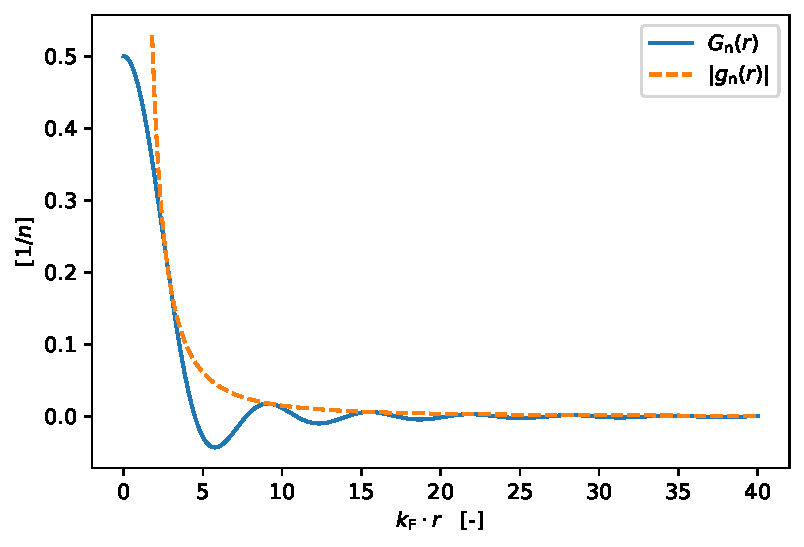
\includegraphics[width=10cm]{G_normal.pdf}
	\caption{A $G_\text{n}(\RR)$ és $\left| g_\text{n}(\RR) \right|$ függvények normált értéke $\kF r$ függvényében.}
	\label{G-normal-fig}
\end{figure}


\subsection{A szupravezető állapotbeli korrelációk}

\subsubsection{Az $F(\RR)$ függvény szupravezető beli alakja}

Ugyanúgy, mint korábban, itt is írjuk fel a \eqref{F-G-def} összefüggés alapján a szupravezető állapotban $F(\RR)$ értékét.  A számolás során felhasználjuk a \eqref{u-v-sc} értékeket, illetve a \eqref{cutoff} levágást.
\begin{equation}
\begin{split}
	F(\RR) & = \frac{1}{V} {\sum\limits_\KK}^\prime e^{-i \KK \RR} u_\KK v_\KK^* = \int \frac{\dd[3]k}{\left( 2 \pi \right)^3} ~ e^{-i \KK \RR} u_\KK v_\KK^* \cdot \frac{1}{\left( \frac{\xi_\KK}{\omega_\text{D}} \right)^4 + 1} = \\
	& = \int\limits_0^{2 \pi} \dd{\varphi} \int\limits_0^\pi \dd{\vartheta} \int\limits_0^\infty \frac{\dd{k}}{\left( 2 \pi \right)^3} ~ k^2 \sin\vartheta ~ e^{-i k r \cos\vartheta} \frac{\Delta^*}{2 \sqrt{\left| \Delta \right|^2 + \xi^2}} \cdot \frac{1}{\left( \frac{\xi}{\omega_\text{D}} \right)^4 + 1} = \\
	& = \frac{1}{2 \pi^2} \, \frac{1}{r} \Im{ \int\limits_0^\infty \dd{k} ~ k \, e^{i k r} \frac{\Delta^*}{2 \sqrt{\left| \Delta \right|^2 + \xi^2}} \cdot \frac{1}{\left( \frac{\xi}{\omega_\text{D}} \right)^4 + 1} }
\end{split}
\end{equation}
Mivel a Fermi-felülethez közeli tartományon integrálunk, közelíthetjük a kitevőben lévő $k$ értékét az alábbi módon,
\begin{equation} \label{k-xi-approx}
	k = \sqrt{2 m \left( \EF + \xi \right)} \approx \kF + \frac{\xi}{\vF},
\end{equation}
ahol $\vF = \frac{\kF}{m}$ a Fermi-sebesség.

A integrálban tényezőként lévő $k$ értékét egyszerűen $\kF$-el közelítjük, mert a pontosabb közelítésből csak egy elhanyagolható nagyságú korrekció származna.

Még érdemes bevezetni a $\Delta$ és $\omega_\text{D}$ energiákhoz tartozó hosszskálákat, a szupravezető korrelációs hosszat és a Debeye hullámhosszat,
\begin{equation}
	\xic \equiv \frac{\vF}{\left| \Delta \right|} ~~~ \text{és} ~~~ \lambda_\text{D} \equiv \frac{\vF}{\omega_\text{D}},
\end{equation}
illetve az $r$ és $\lambda_\text{D}$ szupravezető korrelációs hosszhoz viszonyított értékét,
\begin{equation}
	\tilde{r} \equiv \frac{r}{\xic} ~~~ \text{és} ~~~ \tilde{\lambda}_\text{D} \equiv \frac{\lambda_\text{D}}{\xic}.
\end{equation}

Mindezeket felhasználva
\begin{equation}
	F(\RR) \approx \frac{1}{2 \pi^2} \, \frac{1}{\vF r} \Im{ \int\limits_{-\infty}^\infty \dd{\xi} ~ \kF \, e^{i \kF r} e^{i \, \xi \frac{r}{\vF}} \frac{\Delta^*}{2 \sqrt{\left| \Delta \right|^2 + \xi^2}} \cdot \frac{1}{\left( \frac{\xi}{\omega_\text{D}} \right)^4 + 1} }.
\end{equation}
Az integrált az $x = \frac{\xi}{\left| \Delta \right|}$ változó szerint átírva a következő kifejezést kapjuk,
\begin{equation} \label{f-def}
	F(\RR) \approx \frac{1}{2 \pi^2} \, \frac{1}{\vF r} \Im{ e^{i \kF r} \frac{\Delta^*}{\left| \Delta \right|} \int\limits_{-\infty}^\infty \dd{x} ~ e^{i \tilde{r} x} \frac{1}{2 \sqrt{1 + x^2}} \cdot \frac{1}{\left( \tilde{\lambda}_\text{D} x \right)^4 + 1} }.
\end{equation}
A továbbiakban jelöljük az itt megjelenő integrált $I$-vel.  Ha az integrált kiterjesztjük a komplex síkra azt látjuk, hogy a $\sqrt{1 + x^2}$ miatt a képzetes tengely mentén az integrandusnak szakadása van, illetve a $\frac{1}{\left( \tilde{\lambda}_\text{D} x \right)^4 + 1}$ tényező miatt négy pontban pólusok jelennek meg.  Az integrálási görbét transzformáljuk úgy, hogy az a képzetes tengely menti szakadást körülvegye.  Az integrálási változót $x = i y$ szerint transzformálva az integrál
\begin{equation}
	I = \int\limits_1^\infty \dd{y} ~ \frac{1}{\sqrt{y^2 - 1}} \, e^{-\tilde{r} y} \frac{1}{\left( \tilde{\lambda}_\text{D} y \right)^4 + 1} + R_1 + R_2,
\end{equation}
ahol $R_1$ és $R_2$ az $x_1 = \frac{i + 1}{\sqrt{2} \tilde{\lambda}_\text{D}}$ és $x_2 = \frac{i - 1}{\sqrt{2} \tilde{\lambda}_\text{D}}$ pont beli reziduumok járulékát jelöli.

A reziduumok járulékát könnyen felírhatjuk,
\begin{equation}
	R_1 = 2 \pi i \, e^{i \tilde{r} x_1} \frac{1}{2 \sqrt{1 + x_1^2}} \cdot \frac{1}{4 \tilde{\lambda}_\text{D}^4 x_1^3} \approx -\frac{i \pi}{4} \exp(i \frac{\tilde{r}}{\sqrt{2} \tilde{\lambda}_\text{D}}) \exp(-\frac{\tilde{r}}{\sqrt{2} \tilde{\lambda}_\text{D}})
\end{equation}
és
\begin{equation}
	R_2 = 2 \pi i \, e^{i \tilde{r} x_2} \frac{1}{2 \sqrt{1 + x_2^2}} \cdot \frac{1}{4 \tilde{\lambda}_\text{D}^4 x_2^3} \approx \frac{i \pi}{4} \exp(-i \frac{\tilde{r}}{\sqrt{2} \tilde{\lambda}_\text{D}}) \exp(-\frac{\tilde{r}}{\sqrt{2} \tilde{\lambda}_\text{D}}).
\end{equation}
A kettő összege
\begin{equation}
	R_1 + R_2 \approx \frac{\pi}{2} \exp(-\frac{\tilde{r}}{\sqrt{2} \tilde{\lambda}_\text{D}}) \cos(\frac{\tilde{r}}{\sqrt{2} \tilde{\lambda}_\text{D}}).
\end{equation}

A képzetes tengely menti integrál értékét vizsgáljuk meg $\tilde{r} \gg \tilde{\lambda}_\text{D}$ és $\tilde{r} \ll \tilde{\lambda}_\text{D}$ esetekben.  Az $\tilde{r} \gg \tilde{\lambda}_\text{D}$ távoltéri közelítésben az integrálból kihagyhatjuk a levágást, mivel az exponenciális rész sokkal gyorsabban vág le.  Ezzel az integrált meghatározhatjuk,
\begin{equation}
	I \approx \int\limits_1^\infty \dd{y} ~ \frac{1}{\sqrt{y^2 - 1}} \, e^{-\tilde{r} y} = K_0(\tilde{r}),
\end{equation}
ahol $K_n(x)$ a másodfajú módosított Bessel-függvényeket jelöli.  A reziduumok járuléka $\exp(-\frac{\tilde{r}}{\sqrt{2} \tilde{\lambda}_\text{D}})$ szerint cseng le távoltérben, ami sokkal gyorsabb, mint $K_0(\tilde{r} \gg 1) \sim \frac{\exp(-\tilde{r})}{\sqrt{\tilde{r}}}$ lecsengése, tehát itt azoktól is eltekinthetünk.  Így végül távoltérben az $F(\RR)$ függvény alakja
\begin{equation}
	F(\RR \gg \lambda_\text{D}) \approx \frac{1}{2 \pi^2} \, \frac{1}{\vF r} \cdot K_0(\tilde{r}) \cdot \sin(\kF r).
\end{equation}
A függvény aszimptotikus viselkedését is meghatározhatjuk ebből,
\begin{equation}
	F(\RR \gg \xic) \approx \frac{1}{2 \pi^2} \, \frac{1}{\vF r} \sqrt{\frac{\pi}{2 \tilde{r}}} \cdot e^{-\tilde{r}} \cdot \sin(\kF r).
\end{equation}

Az $\tilde{r} \ll \tilde{\lambda}_\text{D}$ közeltéri közelítésben az integrálban lévő exponenciális függvényt sorba fejthetjük $\tilde{r}$ szerint,
\begin{multline} \label{f-near-field}
	\int\limits_1^\infty \dd{y} ~ \frac{1}{\sqrt{y^2 - 1}} \left( 1 - \tilde{r} y \right) \frac{1}{\left( \tilde{\lambda}_\text{D} y \right)^4 + 1} = \\
	= \int\limits_1^\infty \dd{y} ~ \frac{1}{\sqrt{y^2 - 1}} \cdot \frac{1}{\left( \tilde{\lambda}_\text{D} y \right)^4 + 1} - \tilde{r} \int\limits_1^\infty \dd{y} ~ \frac{y}{\sqrt{y^2 - 1}} \cdot \frac{1}{\left( \tilde{\lambda}_\text{D} y \right)^4 + 1},
\end{multline}
és kapott integrálokat numerikusan könnyen kiértékelhetjük.

A $G_\text{n}(\RR)$ számolásához hasonlóan itt is bevezethetünk egy $f(r)$ komplex mennyiséget, ami az $F(\RR)$ függvény burkolóját jellemzi.  A \eqref{f-def} összefüggés alapján felírhatjuk, hogy
\begin{equation}
	f(r) = \frac{1}{2 \pi^2} \, \frac{\kF}{\xic r} \, \frac{\Delta^*}{\left| \Delta \right|} \cdot I \approx \frac{1}{2 \pi^2} \, \frac{\kF}{\xic r} \, \frac{\Delta^*}{\left| \Delta \right|} \cdot \left\{ \begin{array}{cl}
		K_0(r / \xic), & \text{ha } r \gg \lambda_\text{D} \\
		A - B \cdot r / \xic + R_1 + R_2, & \text{ha } r \ll \lambda_\text{D}
	\end{array} \right. ,
\end{equation}
ahol $A$ és $B$ az \eqref{f-near-field} összefüggésben szereplő integrálok értékei.  Ezzel az $F(\RR)$ függvény
\begin{equation}
\begin{split}
	F(\RR) & = \Im{e^{i \kF r} \cdot f(r)} \approx \\
	& \approx \frac{1}{2 \pi^2} \, \frac{\kF}{\xic r} \, \Im{\frac{\Delta^*}{\left| \Delta \right|} \cdot e^{i \kF r}} \cdot \left\{ \begin{array}{cl}
		K_0(r / \xic), & \text{ha } r \gg \lambda_\text{D} \\
		A - B \cdot r / \xic + R_1 + R_2, & \text{ha } r \ll \lambda_\text{D}
	\end{array} \right. .
\end{split}
\end{equation}

Az analitikus eredmények ellenőrzésére a \eqref{f-def} összefüggés alapján numerikusan is kiszámoltuk $f(r)$ értékét, és összehasonlítottuk a kapott közelítések értékével.  A számolás során a $\left| \Delta \right| : \omega_\text{D} : \EF = 1 : 100 : 10000$ energia arányokat használtuk.  A kapott függvényeket a \ref{F-sc-fig}.\ ábrán láthatjuk.  Az ábrázoláshoz log-log skálát használtunk, hogy jobban elkülönüljenek a görbék.

Az ábrázolt görbéken azt látjuk, hogy a közel- és távoltéri közelítések jól illeszkednek a numerikus eredményhez a megfelelő tartományokban.  Ezt úgy is ellenőrizhetjük, hogy a közelítő függvények relatív eltérését ábrázoljuk $r$ függvényében.  Az eltérés meghatározásához használt képlet távoltéri esetben
$$ \delta f_{r \gg \lambda_\text{D}}(r) = \left| \frac{f(r) - f_{r \gg \lambda_\text{D}}(r)}{f(r)} \right|, $$
és közeltéri esetben is egy ugyanilyen képletet használtunk.  A relatív eltéréseket a \ref{F-sc-error-fig}.\ ábrán láthatjuk.

\begin{figure}[h!]
	\centering
	\begin{subfigure}{0.48\linewidth}
		\centering
		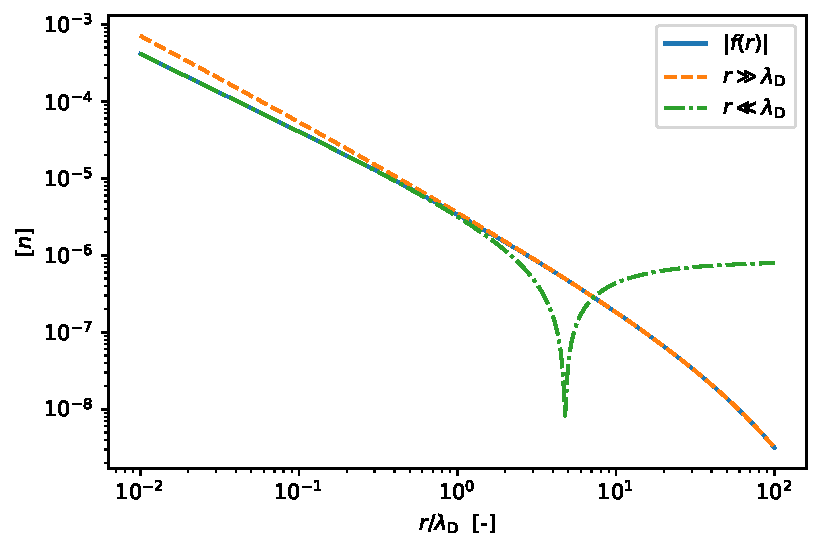
\includegraphics[width=\linewidth]{F_sc.pdf}
		\caption{\centering Az $\left| f(r) \right|$ értéke $r$ függvényében, illetve a közel- és távoltéri közelítő függvények.}
		\label{F-sc-fig}
	\end{subfigure}%
	\begin{subfigure}{0.48\linewidth}
		\centering
		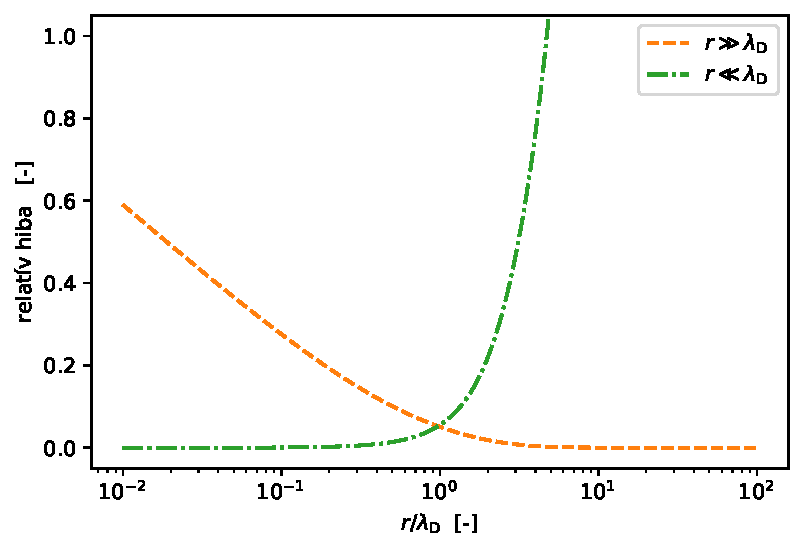
\includegraphics[width=0.98\linewidth]{F_sc_error.pdf}
		\caption{\centering Az $f(r)$-t közelítő függvények relatív hibája $r$ függvényében.}
		\label{F-sc-error-fig}
	\end{subfigure}
	\caption{}
\end{figure}


\subsubsection{A $G(\RR)$ függvény szupravezető beli alakja}

A $G(\RR)$ függvény szupravezető beli alakjának kiszámolásához két mennyiséget kell meghatároznunk.  Először a $\tilde{G}_\text{n}(\RR)$ függvényt, ami a normál állapotban lévő $G_\text{n}(\RR)$ függvénynek a levágással vett járuléka, a $\tilde{G}_\text{SC}(\RR)$ függvényt, ami a szupravezető állapotban a levágással számolt járulék.  Ezekkel a függvényekkel ezután kifejezhetjük a szupravezető állapotban a teljes $G(\RR)$ függvényt,
\begin{equation}
	G(\RR) = G_\text{n}(\RR) - \tilde{G}_\text{n}(\RR) + \tilde{G}_\text{SC}(\RR).
\end{equation}

A $\tilde{G}_\text{n}(\RR)$ járulék kiszámolásánál hasonlóan járunk el, mint korábban,
\begin{equation}
	\tilde{G}_\text{n}(\RR) = \int\limits_{\left| \KK \right| < \kF} \frac{\dd[3]{k}}{\left( 2 \pi \right)^3} ~ e^{-i \KK \RR} \cdot \frac{1}{\left( \frac{\xi_\KK}{\omega_\text{D}} \right)^4 + 1} = \frac{1}{2 \pi^2} \, \frac{1}{r} \Im{ \int\limits_0^{\kF} \dd{k} ~ k \, e^{i k r} \cdot \frac{1}{\left( \frac{\xi}{\omega_\text{D}} \right)^4 + 1} }.
\end{equation}
Itt is elvégezhetjük a \eqref{k-xi-approx} közelítést azzal a különbséggel, hogy a szorzó tényezőként megjelenő $k$ értékét is pontosabbal közelítjük.  Erre azért van szükség, mert az integrál vezető rendet követő tagjait is pontosan kell közelítenünk.  A közelítő mennyiségeket behelyettesítve
\begin{equation}
	\tilde{G}_\text{n}(\RR) = \frac{1}{2 \pi^2} \, \frac{1}{\vF r} \Im{ \int\limits_{-\infty}^0 \dd{\xi} ~ \left( \kF + \frac{\xi}{\vF} \right) e^{i \kF r} e^{i \, \xi \frac{r}{\vF}} \cdot \frac{1}{\left( \frac{\xi}{\omega_\text{D}} \right)^4 + 1} }.
\end{equation}
Az integrált $x = \frac{\xi}{\left| \Delta \right|}$ változó szerint átírva így
\begin{equation}
	\tilde{G}_\text{n}(\RR) = \frac{1}{2 \pi^2} \, \frac{\kF}{\xic r} \Im{ e^{i \kF r} \int\limits_{-\infty}^0 \dd{x} ~ \left( 1 + \frac{x}{\kF \xic} \right) e^{i \tilde{r} x} \cdot \frac{1}{\left( \tilde{\lambda}_\text{D} x \right)^4 + 1} }.
\end{equation}
A továbbiakban jelöljük az itt megjelenő integrált $I_\text{n}$-el.  Hasonlóan az $F(\RR)$ számolásához itt is transzformáljuk az integrálási görbét a komplex síkon úgy, hogy a képzetes tengely mentén integráljunk.  Most is megjelenik egy reziduum az $x_2 = \frac{i - 1}{\sqrt{2} \tilde{\lambda}_\text{D}}$ pontban, így $I_\text{n}$ értéke
\begin{equation}
	I_\text{n} = \int\limits_0^\infty \dd{y} ~ \left( -i + \frac{y}{\kF \xic} \right) e^{-\tilde{r} y} \cdot \frac{1}{\left( \tilde{\lambda}_\text{D} y \right)^4 + 1} + R_{2 \text{n}},
\end{equation}
ahol
\begin{equation}
	R_{2 \text{n}} = 2 \pi i \left( 1 + \frac{x_2}{\kF \xic} \right) e^{i \tilde{r} x_2} \cdot \frac{1}{4 \tilde{\lambda}_\text{D}^4 x_2^3} = \left( -\frac{i \pi}{2} - \frac{\pi}{2 \kF \xic \tilde{\lambda}_\text{D}^2} \right) \exp(-i \frac{\tilde{r}}{\sqrt{2} \tilde{\lambda}_\text{D}}) \exp(-\frac{\tilde{r}}{\sqrt{2} \tilde{\lambda}_\text{D}}).
\end{equation}

Vizsgáljuk meg az integrál értékét $\tilde{r} \gg \tilde{\lambda}_\text{D}$ és $\tilde{r} \ll \tilde{\lambda}_\text{D}$ közelítések mellett is.  Az $\tilde{r} \gg \tilde{\lambda}_\text{D}$ távoltéri közelítésben a levágást elhanyagolhatjuk, tehát az integrál értéke
\begin{equation} \label{g-n-far-field}
	\int\limits_0^\infty \dd{y} ~ \left( -i + \frac{y}{\kF \xic} \right) e^{-\tilde{r} y} = -\frac{i}{\tilde{r}} + \frac{1}{\kF \xic \tilde{r}^2},
\end{equation}
míg az $\tilde{r} \ll \tilde{\lambda}_\text{D}$ közeltéri közelítésben az exponenciális tagot sorba fejthetjük, tehát az integrál értéke
\begin{multline} \label{g-n-near-field}
	\int\limits_0^\infty \dd{y} ~ \left( -i + \frac{y}{\kF \xic} \right) \left( 1 - \tilde{r} y \right) \cdot \frac{1}{\left( \tilde{\lambda}_\text{D} y \right)^4 + 1} = \\
	= \frac{-i \pi}{2 \sqrt{2} \tilde{\lambda}_\text{D}} + \frac{\pi}{4 \kF \xic \tilde{\lambda}_\text{D}^2} - \tilde{r} \cdot \left( \frac{-i \pi}{4 \tilde{\lambda}_\text{D}^2} + \frac{\pi}{2 \sqrt{2} \kF \xic \tilde{\lambda}_\text{D}^3} \right)
\end{multline}

A szupravezető állapot $\tilde{G}_\text{SC}(\RR)$ járuléka is hasonlóan számítható, a levezetésben annyi különbség van, hogy a \eqref{k-xi-approx} közelítést nem alkalmazzuk az integrálban tényezőként megjelenő $k$-ra.  Az $x = \frac{\xi}{\left| \Delta \right|}$ változó szerint felírt integrállal a $G_\text{SC}(\RR)$ függvény értéke
\begin{equation}
	\tilde{G}_\text{SC}(\RR) \approx \frac{1}{2 \pi^2} \, \frac{\kF}{\xic r} \Im{ e^{i \kF r} \int\limits_{-\infty}^\infty \dd{x} ~ \frac{\sqrt{1 + x^2} - x}{2 \sqrt{1 + x^2}} \, e^{i \tilde{r} x} \cdot \frac{1}{\left( \tilde{\lambda}_\text{D} x \right)^4 + 1} }.
\end{equation}
A továbbiakban jelöljük a zárójel beli integrált $I_\text{SC}$-vel.  Hasonlóan a korábbi számításokhoz, itt is transzformáljuk az integrálási görbét úgy, hogy a képzetes tengely mentén integráljunk.  Az integrál értéke
\begin{equation}
	I_\text{SC} = \int\limits_1^\infty \dd{y} ~ \frac{y}{\sqrt{y^2 - 1}} \, e^{-\tilde{r} y} \cdot \frac{1}{\left( \tilde{\lambda}_\text{D} y \right)^4 + 1} + R_{1 \text{SC}} + R_{2 \text{SC}}
\end{equation}
lesz, ahol $R_{1 \text{SC}}$ és $R_{2 \text{SC}}$ az $x_1 = \frac{i + 1}{\sqrt{2} \tilde{\lambda}_\text{D}}$ és $x_2 = \frac{i - 1}{\sqrt{2} \tilde{\lambda}_\text{D}}$ pontokban lévő reziduumok járuléka,
\begin{equation}
	R_{1 \text{SC}} = 2 \pi i \left( \frac{1}{2} - \frac{x_1}{2 \sqrt{1 + x_1^2}} \right) e^{i \tilde{r} x_1} \cdot \frac{1}{4 \tilde{\lambda}_\text{D}^4 x_1^3} \approx \frac{i \pi}{4 x_1} \exp(i \frac{\tilde{r}}{\sqrt{2} \tilde{\lambda}_\text{D}}) \exp(-\frac{\tilde{r}}{\sqrt{2} \tilde{\lambda}_\text{D}}),
\end{equation}
és
\begin{equation}
	R_{2 \text{SC}} = 2 \pi i \left( \frac{1}{2} - \frac{x_2}{2 \sqrt{1 + x_2^2}} \right) e^{i \tilde{r} x_2} \cdot \frac{1}{4 \tilde{\lambda}_\text{D}^4 x_2^3} \approx -\frac{i \pi x_2}{2} \exp(-i \frac{\tilde{r}}{\sqrt{2} \tilde{\lambda}_\text{D}}) \exp(-\frac{\tilde{r}}{\sqrt{2} \tilde{\lambda}_\text{D}}).
\end{equation}
A kettő összege
\begin{equation}
	R_{1 \text{SC}} + R_{2 \text{SC}} \approx R_{2 \text{SC}} = \frac{\pi \left( 1 + i \right)}{2 \sqrt{2} \tilde{\lambda}_\text{D}} \exp(-i \frac{\tilde{r}}{\sqrt{2} \tilde{\lambda}_\text{D}}) \exp(-\frac{\tilde{r}}{\sqrt{2} \tilde{\lambda}_\text{D}}).
\end{equation}

A képzetes tengely menti integrál értékét itt is vizsgáljuk meg $\tilde{r} \gg \tilde{\lambda}_\text{D}$ és $\tilde{r} \ll \tilde{\lambda}_\text{D}$ tartományokban.  Távoltéri közelítésben az integrálból kihagyhatjuk a levágást, mivel az exponenciális rész sokkal gyorsabban vág le. Ezzel az integrál értéke
\begin{equation} \label{g-sc-far-field}
	\int\limits_1^\infty \dd{y} ~ \frac{y}{\sqrt{y^2 - 1}} \, e^{-\tilde{r} y} = K_1(\tilde{r}).
\end{equation}

Közeltéri közelítésben az integrálban lévő exponenciális függvényt sorba fejthetjük $\tilde{r}$ szerint,
\begin{multline} \label{g-sc-near-field}
	\int\limits_1^\infty \dd{y} ~ \frac{y}{\sqrt{y^2 - 1}} \left( 1 - \tilde{r} y \right) \frac{1}{\left( \tilde{\lambda}_\text{D} y \right)^4 + 1} = \\
	= \int\limits_1^\infty \dd{y} ~ \frac{y}{\sqrt{y^2 - 1}} \cdot \frac{1}{\left( \tilde{\lambda}_\text{D} y \right)^4 + 1} - \tilde{r} \int\limits_1^\infty \dd{y} ~ \frac{y^2}{\sqrt{y^2 - 1}} \cdot \frac{1}{\left( \tilde{\lambda}_\text{D} y \right)^4 + 1},
\end{multline}
és a kapott integrálokat numerikusan kiértékelhetjük.

A már korábban bevezetett $g_\text{n}(r)$-hez hasonlóan itt is definiálhatunk burkoló mennyiségeket,
\begin{equation}
	\tilde{g}_\text{n}(r) = \frac{1}{2 \pi^2} \, \frac{\kF}{\xic r} \cdot I_\text{n}, ~~~
	\tilde{g}_\text{SC}(r) = \frac{1}{2 \pi^2} \, \frac{\kF}{\xic r} \cdot I_\text{SC},
\end{equation}
és a teljes $G(\RR)$ függvény $g(r)$ burkolóját kifejezhetjük ezekkel,
\begin{equation}
	g(r) = g_\text{n}(r) - \tilde{g}_\text{n}(r) + \tilde{g}_\text{SC}(r).
\end{equation}
Vizsgáljuk meg ennek a függvénynek a távol- és közeltéri értékeit.  Távoltérben a \eqref{g-n-far-field} és \eqref{g-sc-far-field} összefüggéseket használhatjuk,
\begin{equation}
\begin{split}
	g(r \gg \lambda_\text{D}) & \approx \frac{1}{2 \pi^2} \cdot \left( \frac{1 - i \kF r}{r^3} - \frac{\kF}{\xic r} \cdot \left( -\frac{i}{\tilde{r}} + \frac{1}{\kF \xic \tilde{r}^2} \right) + \frac{\kF}{\xic r} \cdot K_1(\tilde{r}) \right) \approx \\
	& \approx \frac{1}{2 \pi^2} \, \frac{\kF}{\xic r} \cdot K_1(r / \xic).
\end{split}
\end{equation}
Azt látjuk, hogy távoltérben a $g_\text{n}(r)$ teljesen kiesik, és csak a szupravezető járulék marad meg,
\begin{equation}
	g(r \gg \lambda_\text{D}) \approx \frac{1}{2 \pi^2} \, \frac{\kF}{\xic r} \cdot K_1(r / \xic),
\end{equation}
ezzel a $G(\RR)$ függvényt felírva
\begin{equation}
	G(\RR \gg \lambda_\text{D}) \approx \frac{1}{2 \pi^2} \, \frac{\kF}{\xic r} \cdot K_1(\tilde{r}) \cdot \sin(\kF r).
\end{equation}
A függvény aszimptotikus viselkedését is meghatározhatjuk ebből,
\begin{equation}
	G(\RR \gg \xic) \approx \frac{1}{2 \pi^2} \, \frac{\kF}{\xic r} \sqrt{\frac{\pi}{2 \tilde{r}}} \cdot e^{-\tilde{r}} \cdot \sin(\kF r)
\end{equation}

Közeltérben a \eqref{g-n-near-field} és \eqref{g-sc-near-field} összefüggéseket használhatjuk,
\begin{equation} \label{g-near-field}
	g(r \ll \lambda_\text{D}) \approx \frac{1}{2 \pi^2} \cdot \left( \frac{1 - i \kF r}{r^3} + \frac{\kF}{\xic r} \cdot \left( A - B \cdot r / \xic - R_{2 \text{n}} + R_{1 \text{SC}} + R_{2 \text{SC}} \right) \right),
\end{equation}
ahol $A$ és $B$ az egyes eseteknél számolt együtthatók különbsége.

Végül $g(r)$ segítségével felírhatjuk a $G(\RR)$ függvény alakját,
\begin{equation}
	G(\RR \gg \lambda_\text{D}) \approx \frac{1}{2 \pi^2} \cdot \frac{\kF}{\xic r} \cdot K_1(r / \xic) \cdot \sin(\kF r),
\end{equation}
és
\begin{multline}
	G(\RR \ll \lambda_\text{D}) \approx \frac{1}{2 \pi^2} \cdot \left( \frac{\sin(\kF r) - \kF r \cos(\kF r)}{r^3} +
	\right. \\ \left. +
	\frac{\kF}{\xic r} \cdot \sin(\kF r) \cdot \left( A - B \cdot r / \xic - R_{2 \text{n}} + R_{1 \text{SC}} + R_{2 \text{SC}} \right) \right)
\end{multline}

Az eredmények ellenőrzésére $g(r)$ értékét numerikusan is kiszámoltuk, és összehasonlítottuk a kapott közelítések értékével.  A számolás során a $\left| \Delta \right| : \omega_\text{D} : \EF = 1 : 100 : 10000$ energia arányokat használtuk.  A kapott függvényeket az \ref{G-sc-fig}.\ ábrán láthatjuk.  Az ábrázoláshoz log-log skálát használtunk.

\begin{figure}[h!]
	\centering
	\begin{subfigure}{0.48\linewidth}
		\centering
		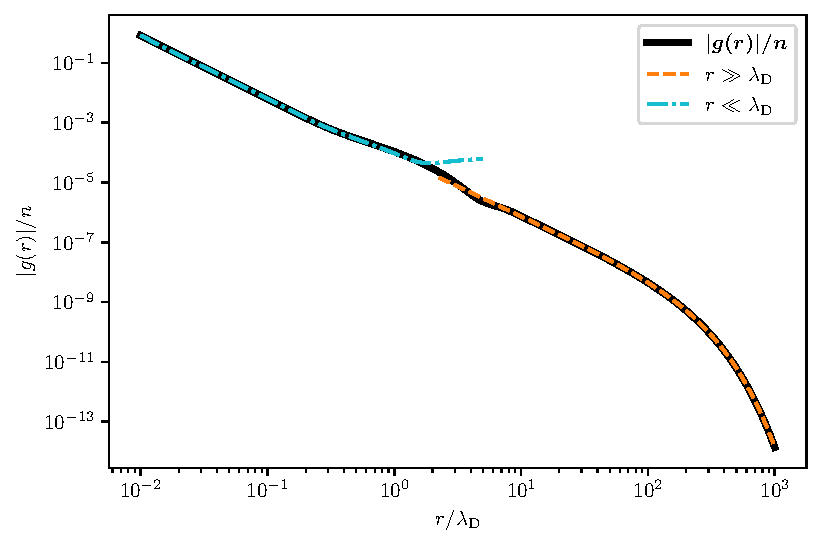
\includegraphics[width=\linewidth]{G_sc.pdf}
		\caption{\centering A $\left| g(r) \right|$ értéke $r$ függvényében, illetve a közel- és távoltéri közelítő függvények.}
		\label{G-sc-fig}
	\end{subfigure}
	\begin{subfigure}{0.48\linewidth}
		\centering
		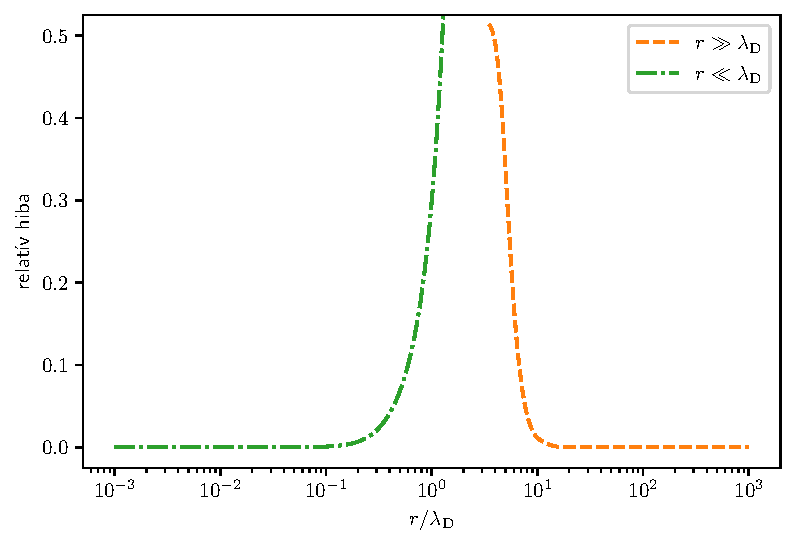
\includegraphics[width=0.98\linewidth]{G_sc_error.pdf}
		\caption{\centering A $g(r)$-t közelítő függvények relatív hibája $r$ függvényében.}
		\label{G-sc-error-fig}
	\end{subfigure}
	\caption{}
\end{figure}

Az ábrázolt görbéken azt látjuk, hogy a közel- és távoltéri közelítések jól illeszkednek a numerikus eredményhez a megfelelő tartományokban.  Ezt úgy is ellenőrizhetjük, hogy a közelítő függvények $g(r)$-től való relatív eltérését kiszámoljuk.  Az eltérés meghatározásához használt képlet távoltéri esetben
$$ \delta g_{r \gg \lambda_\text{D}}(r) = \left| \frac{g(r) - g_{r \gg \lambda_\text{D}}(r)}{g(r)} \right|, $$
és közeltéri esetben is egy ugyanilyen képletet használtunk.  A relatív eltéréseket az \ref{G-sc-error-fig}.\ ábrán láthatjuk.



% ================================================================
\section{Spin- és töltéskorrelációs függvények}

A spin- és töltéskorrelációs függvényeket már korábban kifejeztük az $F(\RR)$ és $G(\RR)$ függvények segítségével, így azokat egyszerűen ki tudjuk számolni ezek segítségével.  Itt is érdemes burkoló görbéket számolni.  A $G^2(\RR)$ és $F^2(\RR)$ függvényeket fejezzük ki,
\begin{equation} \label{F2-G2-bound}
\begin{split}
	G^2(\RR) & = \left(\Im{ e^{i \kF r} \cdot g(r) }\right)^2 = \frac{\left| g(r) \right|^2 - \Re{ e^{2 \, i \kF r} \cdot g^2(r) }}{2}, \\
	F^2(\RR) & = \left(\Im{ e^{i \kF r} \cdot f(r) }\right)^2 = \frac{\left| f(r) \right|^2 - \Re{ e^{2 \, i \kF r} \cdot f^2(r) }}{2}.
\end{split}
\end{equation}
Ezeknek a függvényeknek az értékei rendre a $\left[ 0, \left| g(r) \right|^2 \right]$ és $\left[ 0, \left| f(r) \right|^2 \right]$ tartományokban vannak.  A továbbiakban használjuk az alábbi jelölést,
\begin{equation}
\begin{split}
	\expval{\delta\rho(\RR) \delta\rho(0)} & = \Re{g_{\rho 0}(r) - e^{2 \, i \kF r} \cdot g_\rho(r)}, \\
	\expval{\va*{s}(\RR) \cdot \va*{s}(0)} & = \Re{g_{\va*{s} 0}(r) - e^{2 \, i \kF r} \cdot g_{\va*{s}}(r)}.
\end{split}
\end{equation}
Az itt megjelenő burkolókat így könnyen felírhatjuk a \eqref{charge-F-G}, \eqref{spin-F-G} és \eqref{F2-G2-bound} összefüggések segítségével,
\begin{equation} \label{charge-spin-bound}
\begin{split}
	g_{\rho 0}(r) = \left| f(r) \right|^2 - \left| g(r) \right|^2, ~~~ & g_{\va*{s} 0}(r) = \frac{3}{4} \left( -\left| f(r) \right|^2 - \left| g(r) \right|^2 \right), \\
	g_\rho(r) = f^2(r) - g^2(r), ~~~ & g_{\va*{s}}(r) = \frac{3}{4} \left( -f^2(r) - g^2(r) \right).
\end{split}
\end{equation}


\subsection{Korrelációs függvények normál állapotban}

Normál állapotban a $g(r)$ és $f(r)$ függvények pontos alakja ismert,
\begin{equation}
	g_\text{n}(r) = \frac{1}{2 \pi^2} \cdot \frac{1 - i \kF r}{r^3} ~~~ \text{és} ~~~ f_\text{n}(r) = 0.
\end{equation}
Ezekkel kifejezve a korrelációs függvényeket,
\begin{equation}
\begin{split}
	\expval{\delta\rho(\RR) \delta\rho(0)} & = -2 \, G_\text{n}^2(\RR), \\
	\expval{\va*{s}(\RR) \cdot \va*{s}(0)} & = -\frac{3}{2} \, G_\text{n}^2(\RR),
\end{split}
\end{equation}
és behelyettesítve $G_\text{n}(\RR)$ értékét,
\begin{equation}
\begin{split}
	\expval{\delta\rho(\RR) \delta\rho(0)} & = \frac{1}{2 \pi^4} \left( -\frac{1 + \left( \kF r \right)^2}{r^6} + \frac{\left( 1 - \left( \kF r \right)^2 \right) \cdot \cos(2 \, \kF r) + 2 \, \kF r \cdot \sin(2 \, \kF r)}{r^6} \right), \\
	\expval{\va*{s}(\RR) \cdot \va*{s}(0)} & = \frac{3}{8 \pi^4} \left( -\frac{1 + \left( \kF r \right)^2}{r^6} + \frac{\left( 1 - \left( \kF r \right)^2 \right) \cdot \cos(2 \, \kF r) + 2 \, \kF r \cdot \sin(2 \, \kF r)}{r^6} \right).
\end{split}
\end{equation}
Mindkét korrelátor függvény a $-G_\text{n}^2(\RR)$ függvénnyel arányos.  Ezt a függvényt a \ref{G2-normal-fig}.\ ábrán láthatjuk.

\begin{figure}[h!]
	\centering
	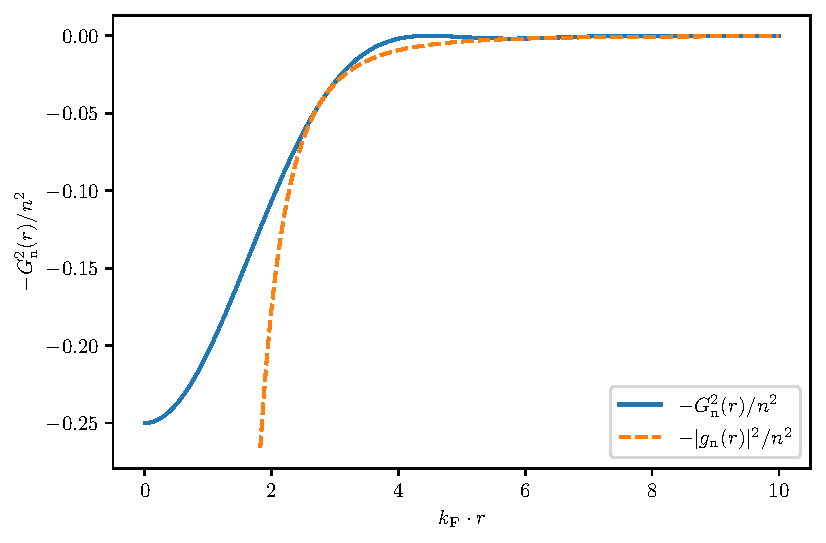
\includegraphics[width=10cm]{G2_normal.pdf}
	\caption{A $G_\text{n}^2(\RR)$ függvény értéke $\RR$ függvényében.}
	\label{G2-normal-fig}
\end{figure}

Az ábrán azt látjuk, hogy a függvény $r = 0$ esetén egy negatív véges értéket vesz föl, egyébként pedig gyorsan lecseng.  Az $r = 0$ helyen lévő lyuk az úgynevezett Pauli-lyuk.  Ez a Pauli-elv következménye, ami szerint nem lehet két elektron egyszerre ugyanabban az állapotban.  Töltéskorreláció esetén ez azt eredményezi, hogy a nagy távolságoknál várt átlagos részecskeszám négyzetéhez képest ennek a fele fog megjelenni, mert az origóban lévő elektron kiszorítja a többit arról a helyről.  Spinkorreláció esetén is hasonló történik.  Mivel az origóban lévő elektron az azonos spinű elektronokat szorítja ki, ezért egy negatív korrelációt kapunk.


\subsection{Töltéskorrelációs függvény}

A töltéskorrelációs függvény burkolóját a \eqref{charge-spin-bound} összefüggés szerint számolhatjuk ki.  Itt is vizsgáljuk az $r \gg \lambda_\text{D}$ és $r \ll \lambda_\text{D}$ tartományokat.  Az $r \gg \lambda_\text{D}$ távoltéri közelítésben
\begin{equation} \label{f2-g2-far}
\begin{split}
	f^2(r) \approx \left| f(r) \right|^2 & \approx \left( \frac{1}{2 \pi^2} \, \frac{\kF}{\xic r} \right)^2 \cdot K_0^2(r / \xic), \\
	g^2(r) \approx \left| g(r) \right|^2 & \approx \left( \frac{1}{2 \pi^2} \, \frac{\kF}{\xic r} \right)^2 \cdot K_1^2(r / \xic),
\end{split}
\end{equation}
így a töltéskorrelációs függvény burkolói
\begin{equation}
	g_{\rho 0}(r \gg \lambda_\text{D}) \approx g_\rho(r \gg \lambda_\text{D}) \approx \left( \frac{1}{2 \pi^2} \, \frac{\kF}{\xic r} \right)^2 \cdot \left( K_0^2(r / \xic) - K_1^2(r / \xic) \right),
\end{equation}
amik $r \gg \xic$ esetén tovább egyszerűsödnek,
\begin{equation}
	g_{\rho 0}(r \gg \xic) \approx g_\rho(r \gg \xic) \approx -\left( \frac{1}{2 \pi^2} \, \frac{\kF}{r} \right)^2 \cdot \frac{\pi}{2 \, r^2} \, \exp(-2 \, r / \xic) \sim -\frac{\exp(-2 \, r / \xic)}{r^4}.
\end{equation}
Ezekkel felírhatjuk a töltéskorrelációs függvény teljes közelítő alakját $r \gg \lambda_\text{D}$ és $r \gg \xic$ esetén,
\begin{equation}
\begin{split}
	\expval{\delta\rho(\RR \gg \lambda_\text{D}) \delta\rho(0)} & \approx \left( \frac{1}{2 \pi^2} \, \frac{\kF}{\xic r} \right)^2 \cdot \left( K_0^2(r / \xic) - K_1^2(r / \xic) \right) \cdot \left( 1 - \cos(2 \, \kF r) \right), \\
	\expval{\delta\rho(\RR \gg \xic) \delta\rho(0)} & \approx \left( \frac{1}{2 \pi^2} \, \frac{\kF}{r} \right)^2 \cdot \frac{\pi}{2 \, r^2} \, \exp(-2 \, r / \xic) \cdot \left( 1 - \cos(2 \, \kF r) \right),
\end{split}
\end{equation}

Az $r \ll \lambda_\text{D}$ közeltéri közelítésben belátható, hogy $\left| f(r) \right|^2 \ll \left| g(r) \right|^2$, így a burkoló függvények
\begin{equation}
	g_{\rho 0}(r \ll \lambda_\text{D}) \approx -\left| g(r) \right|^2 ~~~ \text{és} ~~~ g_\rho(r \ll \lambda_\text{D}) \approx -g^2(r)
\end{equation}
lesznek, ahol $g(r)$ a \eqref{g-near-field} összefüggés alapján írható fel.  Fontos, hogy $g(r)$ szupravezető járulékától nem tekinthetünk el, ellenkező esetben a közelítés rossz lesz $r \gtrsim \kF^{-1}$ esetén.

A korábbiakhoz hasonlóan a korrelációs függvényt numerikusan is ellenőriztük.  A számolás során itt is a $\left| \Delta \right| : \omega_\text{D} : \EF = 1 : 100 : 10000$ energia arányokat használtuk.  Az ábrázolásnál a $\expval{\delta\rho(\RR) \delta\rho(0)}$ korrelációs függvény harmonikus függésének amplitúdóját ábrázoltuk, vagyis $\left| g_\rho(r) \right|$-t, illetve ezek közelítő függvényeit.  Ezen kívül a közelítések relatív hibáit is ábrázoltuk.  Mindezt a \ref{rho-fig}.\ ábrán láthatjuk.  A használt közelítő függvények itt is jól illeszkednek a megfelelő tartományokban a numerikusan számolt görbéhez.

\begin{figure}[H]
	\centering
	\begin{subfigure}[t]{0.48\linewidth}
		\centering
		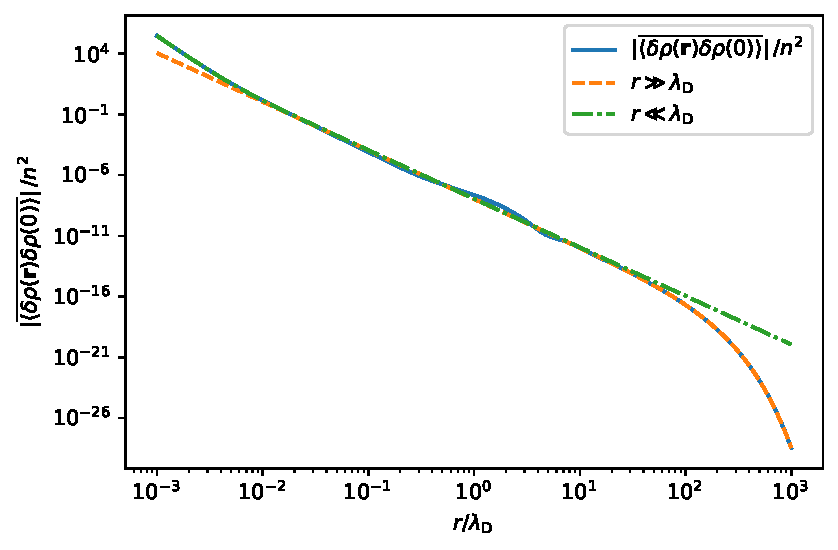
\includegraphics[width=\linewidth]{rho.pdf}
		\caption{\centering A töltéskorrelációs függvény burkoló görbéje az $r$ függvényében, illetve a közel- \newline és távoltéri közelítő függvények.}
	\end{subfigure}%
	\begin{subfigure}[t]{0.48\linewidth}
		\centering
		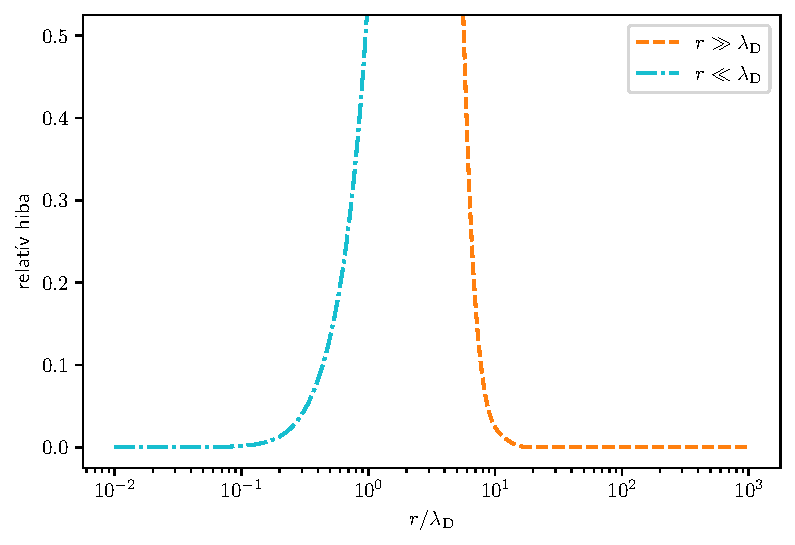
\includegraphics[width=0.96\linewidth]{rho_error.pdf}
		\caption{\centering A töltéskorrelációs függvény burkoló görbéjét közelítő függvények relatív hibája \newline $r$ függvényében.}
	\end{subfigure}
	\caption{}
	\label{rho-fig}
\end{figure}


\subsection{Spinkorrelációs függvény}

A spinkorrelációs függvényt és annak burkolóját a \eqref{charge-spin-bound} összefüggés alapján számolhatjuk ki.  Az $r \gg \lambda_\text{D}$ távoltéri közelítésben \eqref{f2-g2-far} összefüggés teljesül, így a spinkorrelációs függvény burkolói
\begin{equation}
	g_{\va*{s} 0}(r \gg \lambda_\text{D}) \approx g_{\va*{s}}(r \gg \lambda_\text{D}) \approx -\frac{3}{4} \cdot \left( \frac{1}{2 \pi^2} \, \frac{\kF}{\xic r} \right)^2 \cdot \left( K_0^2(r / \xic) + K_1^2(r / \xic) \right),
\end{equation}
amik $r \gg \xic$ esetén tovább egyszerűsödnek,
\begin{equation}
	g_{\va*{s} 0}(r \gg \xic) \approx g_{\va*{s}}(r \gg \xic) \approx -\frac{3}{4} \cdot \left( \frac{1}{2 \pi^2} \, \frac{\kF}{r} \right)^2 \cdot \frac{\pi}{\xic r} \, \exp(-2 \, r / \xic) \sim -\frac{\exp(-2 \, r / \xic)}{r^3}.
\end{equation}
Ezekkel felírhatjuk a spinkorrelációs függvény teljes közelítő alakját $r \gg \lambda_\text{D}$ és $r \gg \xic$ esetén,
\begin{equation}
\begin{split}
	\expval{\va*{s}(\RR \gg \lambda_\text{d}) \cdot \va*{s}(0)} & \approx -\frac{3}{4} \cdot \left( \frac{1}{2 \pi^2} \, \frac{\kF}{\xic r} \right)^2 \cdot \left( K_0^2(r / \xic) + K_1^2(r / \xic) \right) \cdot \left( 1 - \cos(2 \, \kF r) \right), \\
	\expval{\va*{s}(\RR \gg \xic) \cdot \va*{s}(0)} & \approx -\frac{3}{4} \cdot \left( \frac{1}{2 \pi^2} \, \frac{\kF}{r} \right)^2 \cdot \frac{\pi}{\xic r} \, \exp(-2 \, r / \xic) \cdot \left( 1 - \cos(2 \, \kF r) \right).
\end{split}
\end{equation}

Az $r \ll \lambda_\text{D}$ közeltéri közelítésben itt is felhasználhatjuk, hogy $\left| f(r) \right|^2 \ll \left| g(r) \right|^2$, így a burkoló függvények
\begin{equation}
	g_{\va*{s} 0}(r \ll \lambda_\text{D}) \approx -\frac{3}{4} \cdot \left| g(r) \right|^2 ~~~ \text{és} ~~~ g_{\va*{s}}(r \ll \lambda_\text{D}) \approx -\frac{3}{4} \cdot g^2(r)
\end{equation}
lesznek, ahol $g(r)$ a \eqref{g-near-field} összefüggés alapján írható fel.

Itt is csináltunk egy numerikus ellenőrzést ugyanolyan paraméterekkel, mint a töltéskorrelációs függvény esetén.  A $\left| g_{\va*{s}}(r) \right|$ burkoló függvényt a közelítő függvényekkel együtt, illetve a közelítések relatív hibáit a \ref{s-fig}.\ ábrán láthatjuk.  A használt közelítő függvények itt is jól illeszkednek a megfelelő tartományokban.

\begin{figure}[h!]
	\centering
	\begin{subfigure}[t]{0.48\linewidth}
		\centering
		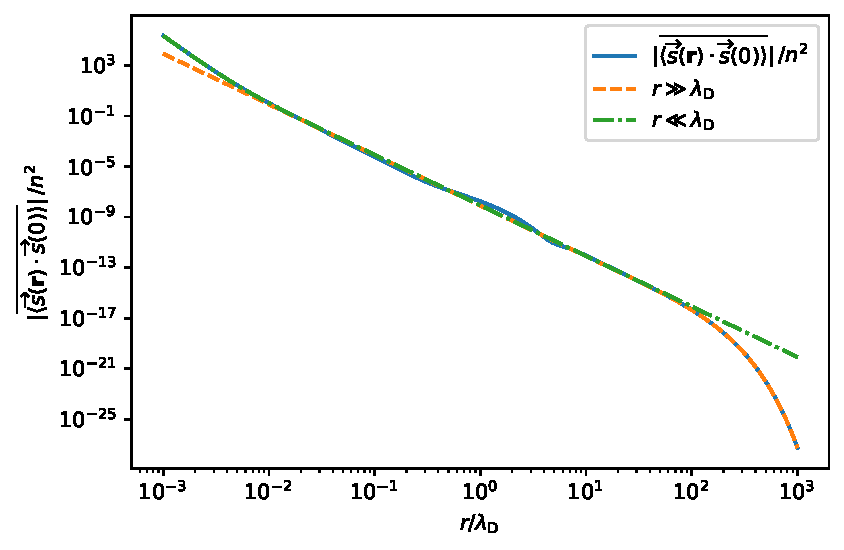
\includegraphics[width=\linewidth]{s.pdf}
		\caption{\centering A spinkorrelációs függvény burkoló görbéje az $r$ függvényében, illetve a közel- \newline és távoltéri közelítő függvények.}
	\end{subfigure}%
	\begin{subfigure}[t]{0.48\linewidth}
		\centering
		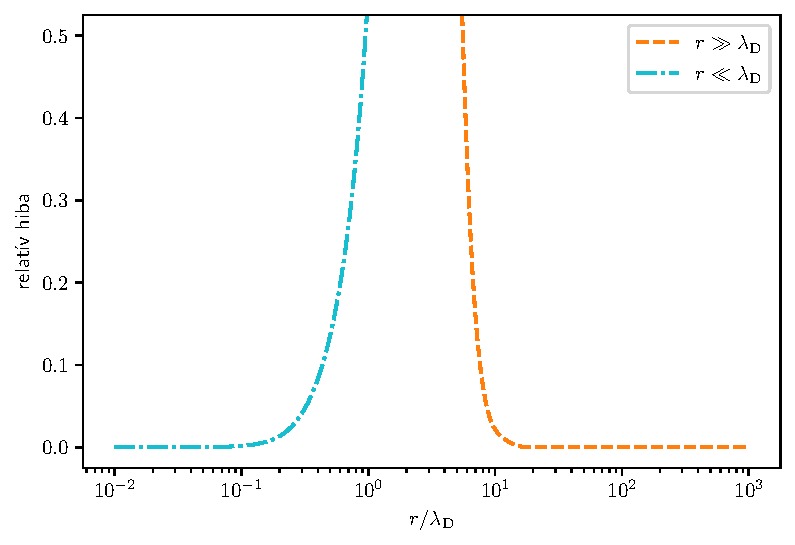
\includegraphics[width=0.96\linewidth]{s_error.pdf}
		\caption{\centering A spinkorrelációs függvény burkoló görbéjét közelítő függvények relatív hibája \newline $r$ függvényében.}
	\end{subfigure}
	\caption{}
	\label{s-fig}
\end{figure}



% ================================================================
\section{Konklúzió}

A dolgozatban megvizsgáltuk, hogy egy szupravezetőben hogyan változnak a spin- és töltéskorrelációs függvények a normál állapothoz képest.  Háromféle hosszskála jelent meg az eredményeinkben, ezek a $\kF$ Fermi-hullámszám, a $\lambda_\text{D} = \frac{\vF}{\omega_\text{D}}$ Debeye-hossz és a $\xic = \frac{\hbar \vF}{\left| \Delta \right|}$ szupravezető korrelációs hossz, ahol $\vF$ a Fermi-sebesség, $\omega_\text{D}$ a Debeye-frekvencia és $\Delta$ a szupravezető gap nagysága.

Azt tapasztaltuk, hogy a korrelációk lokalizáltabbak a szupravezető állapotban.  A szupravezető állapotban lévő spin- és töltéskorrelációs függvények lecsengése vezető rendben aszimptotikusan, az $r \gg \xic$ tartományban rendre $\sim \frac{\exp(-2 \, r / \xic)}{r^3}$ és $\sim \frac{\exp(-2 \, r / \xic)}{r^4}$.  Ezzel szemben a normál állapotban mindkét esetben $\sim r^{-4}$ lecsengést kapunk.  Az exponenciális lecsengés karakterisztikus hossza $\xic$ a szupravezető korrelációs hossz.  Az $r \ll \lambda_\text{D}$ tartományban a szupravezető állapotbeli korrelációs függvények egy $\order{r^{-2}}$ kis korrekción kívül megegyeznek a normál állapotbeli függvényekkel.

A korrelációs függvényekhez analitikus közelítő függvényeket is meghatároztunk $r \ll \lambda_\text{D}$ és $r \gg \lambda_\text{D}$ tartományokban.  Ezek érvényességi tartományát a $\lambda_\text{D}$ Debeye-hossz határozza meg.  Az ehhez tartozó $\omega_\text{D}$ Debeye-frekvenciának az a szerepe a szupravezetésben, hogy a Fermi-felület körül csak a $\pm \hbar \omega_\text{D}$ energiatartományban hatnak kölcsön az elektronok, és rendeződnek Cooper-párokba.  Ennek megfelelően $r \ll \lambda_\text{D}$ esetén lényegében a normál állapotbeli függvényeket kapjuk vissza.  Ezek a vizsgált 3 dimenziós esetben
$$ \expval{\va*{s}(\RR) \cdot \va*{s}(0)}, \ \expval{\delta\rho(\RR) \delta\rho(0)} \sim \frac{\left( \sin(\kF r) - \kF r \cos(\kF r) \right)^2}{r^6} $$
lecsengést mutatnak.

Az $r \approx \lambda_\text{D}$ tartományban nem tudtunk analitikus megoldást adni a korrelációs függvények alakjára.  Itt a szupravezető járulék és a normál állapotbeli korrelációk keverednek, ahogy $r$ nő, a szupravezető járulék egyre dominánsabbá válik.  Habár analitikus megoldás nincs ebben a tartományban, numerikusan jól lehet számolni a két állapot járulékát.

Az $r \gg \lambda_\text{D}$ tartományban az $F(\RR)$ párkorrelációs függvény és a $G(\RR)$ normál korrelációs függvény másodfajú módosított Bessel-függvényeket követnek.  Spinkorrelációs függvénynél a két járulék erősíti egymást,
\begin{equation}
	\expval{\va*{s}(\RR) \cdot \va*{s}(0)} \approx -\frac{3}{4} \cdot \left( \frac{1}{2 \pi^2} \, \frac{\kF}{\xic r} \right)^2 \cdot \left( K_0^2(r / \xic) + K_1^2(r / \xic) \right) \cdot \left( 1 - \cos(2 \, \kF r) \right),
\end{equation}
%	\expval{\va*{s}(\RR \gg \xic) \cdot \va*{s}(0)} & \approx -\frac{3}{4} \cdot \left( \frac{1}{2 \pi^2} \, \frac{\kF}{r} \right)^2 \cdot \frac{\pi}{\xic r} \, \exp(-2 \, r / \xic) \cdot \left( 1 - \cos(2 \, \kF r) \right).
míg töltéskorrelációs függvénynél gyengítik egymást,
\begin{equation}
	e^2 \, \expval{\delta\rho(\RR) \delta\rho(0)} \approx e^2 \left( \frac{1}{2 \pi^2} \, \frac{\kF}{\xic r} \right)^2 \cdot \left( K_0^2(r / \xic) - K_1^2(r / \xic) \right) \cdot \left( 1 - \cos(2 \, \kF r) \right).
\end{equation}
A korrelációs függvények aszimptotikus viselkedése $r \gg \xic$ esetén pedig
\begin{equation}
\begin{split}
	\expval{\va*{s}(\RR \gg \xic) \cdot \va*{s}(0)} & \sim \frac{\exp(-2 \, r / \xic)}{r^3} \cdot \left( 1 - \cos(2 \, \kF r) \right), \\
	\expval{\delta\rho(\RR \gg \xic) \delta\rho(0)} & \sim \frac{\exp(-2 \, r / \xic)}{r^4} \cdot \left( 1 - \cos(2 \, \kF r) \right).
\end{split}
\end{equation}

Az eredményeink akkor érvényesek, ha teljesül a $\kF^{-1} \ll \lambda_\text{D} \ll \xic$ reláció.  Ez a legtöbb közönséges szupravezetőben így van.  Léteznek azonban olyan szupravezetők, amikben a $\Delta_\KK$ gap függvénynek nódusai vannak (pl.\ magas hőmérsékletű szupravezetők).  Ezeknél a számításainkból arra következtethetünk, hogy a korrelációs függvények aszimptotikus viselkedése nem egy exponenciális, hanem valamilyen hatványfüggvényt követ.  Az eredményeink továbbá nem érvényesek olyan szupravezetőkre, amikre nem ismert a BCS-elmélet (pl.\ $\mathrm{U}\mathrm{Be}_{13}$).



\pdfbookmark{Hivatkozások}{bm:hivatkozasok}

\begin{thebibliography}{}

\bibitem{openstax}
OpenStax College: \emph{College Physics} (OpenStax College, 2017) \\
\href{https://openstax.org/details/books/college-physics-ap-courses}{\texttt{https://openstax.org/details/books/college-physics-ap-courses}}

\bibitem{superconductor-gap}
Electric control of superconducting transition through a spin-orbit coupled interface - Scientific Figure on ResearchGate. \newline
\href{https://www.researchgate.net/figure/Sketch-of-the-superconducting-gap-D-as-a-function-of-temperature-T-for-a-superconducting_fig3_305412985}{\texttt{https://www.researchgate.net/figure/Sketch-of-the-superconducting-gap-D- as-a-function-of-temperature-T-for-a-superconducting\_fig3\_305412985}}

\bibitem{ashcroft}
Neil W.\ Ashcroft, N.\ David Mermin: \emph{Solid State Physics} (Saunders College, 1976)

\bibitem{degennes}
P.\ G.\ de Gennes: \emph{Superconductivity of Metals and Alloys}, Advanced Book Classics \newline (Westview Press, 1966)

\end{thebibliography}


\end{document}
